% Компиляция: xelatex courier_lab_report.tex
\documentclass[12pt,a4paper]{article}
\usepackage{fontspec}
\usepackage{polyglossia}
\setdefaultlanguage{russian}
\setotherlanguage{english}
\setmainfont{Times New Roman}
\setmonofont{Courier New}
\newfontfamily\cyrillicfonttt{Courier New}
\usepackage{geometry}
\usepackage{graphicx}
\usepackage{float}
\usepackage{caption}
\usepackage{indentfirst}
\usepackage{array}
\usepackage[hidelinks]{hyperref}
\geometry{left=2.5cm,right=1.5cm,top=2cm,bottom=2cm}
\graphicspath{{../data/}{../results/}}
\captionsetup{font=small,labelsep=period}
\setlength{\parindent}{1.25cm}
\setlength{\parskip}{0pt}
\emergencystretch=2em

\begin{document}
\begin{titlepage}
\begin{center}
Министерство науки и высшего образования Российской Федерации\\
НАЦИОНАЛЬНЫЙ ИССЛЕДОВАТЕЛЬСКИЙ\\
ТОМСКИЙ ГОСУДАРСТВЕННЫЙ УНИВЕРСИТЕТ (НИ ТГУ)\\
Институт прикладной математики и компьютерных наук

\vspace{5cm}
ОТЧЕТ ПО ЛАБОРАТОРНОЙ РАБОТЕ\\[0.3cm]
по дисциплине <<Глубокое обучение>>\\[0.4cm]
{\large Разработка среды с неопределенностью}\\[0.5cm]
Сальников Никита Сергеевич\\[0.3cm]
Направление подготовки 02.03.02\\
Фундаментальная информатика и информационные технологии\\
Направленность (профиль)\\
<<Искусственный интеллект и разработка программных продуктов>>

\vspace{2.5cm}
\begin{flushright}
Руководитель работы\\
кандидат технических наук\\
\begin{tabular}{c l}
\rule{3cm}{0.4pt} & С.В. Аксёнов\\
{\small подпись} &
\end{tabular}\\
<<\rule{0.7cm}{0.4pt}>> \rule{2.5cm}{0.4pt} 2026 г.\\[0.8cm]
Автор работы\\
студент группы № 932301\\
\begin{tabular}{c l}
\rule{3cm}{0.4pt} & Н.С. Сальников\\
{\small подпись} &
\end{tabular}\\
<<\rule{0.7cm}{0.4pt}>> \rule{2.5cm}{0.4pt} 2026 г.
\end{flushright}

\vfill
Томск - 2026
\end{center}
\end{titlepage}

\section{Постановка задачи и карта}
Цель работы - построить среду с неопределённым движением транспорта и сравнить три заданные вручную стратегии курьера. Для карты взят участок Павлодара из OpenStreetMap. Дорожные линии переведены в связную сетку $160\times160$ клеток. Дорожные клетки проходимы в обоих направлениях; остальные клетки считаются препятствиями. Обучение агента в этой работе не выполнялось.

\begin{figure}[H]
\centering
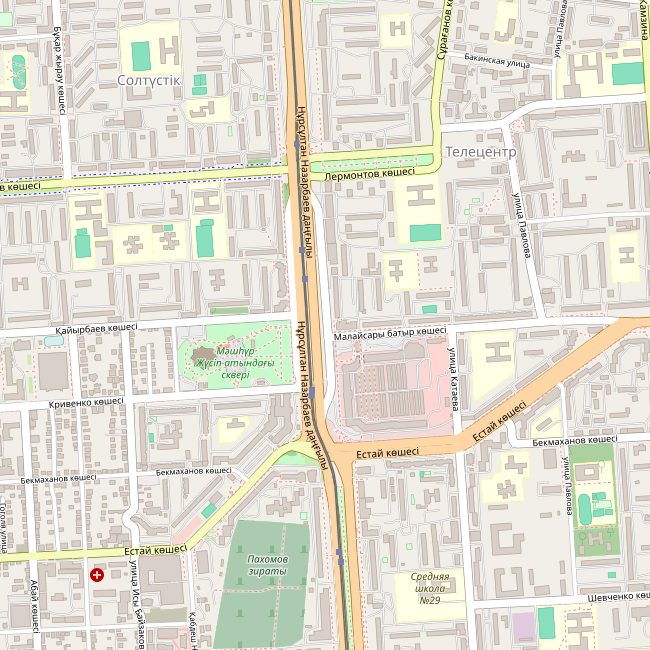
\includegraphics[width=.44\textwidth]{source_osm_map.png}\hfill
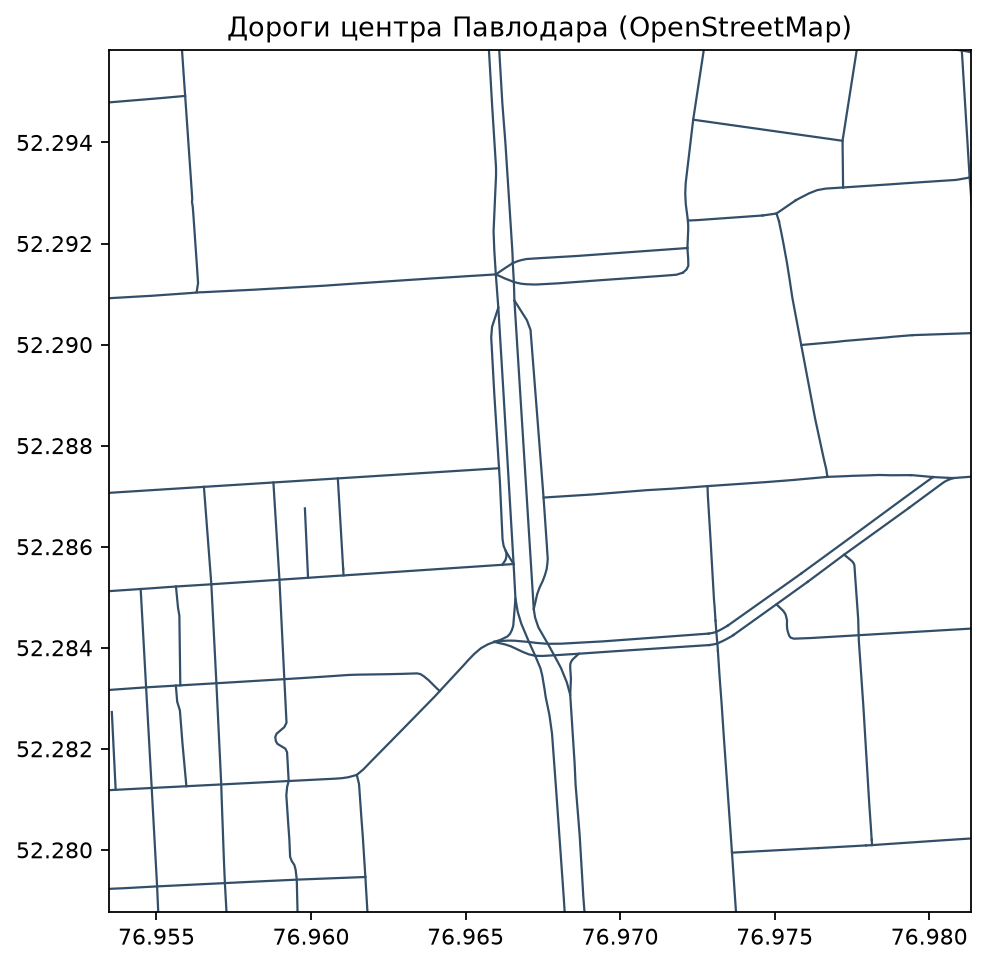
\includegraphics[width=.44\textwidth]{source_roads.png}\\[0.3cm]
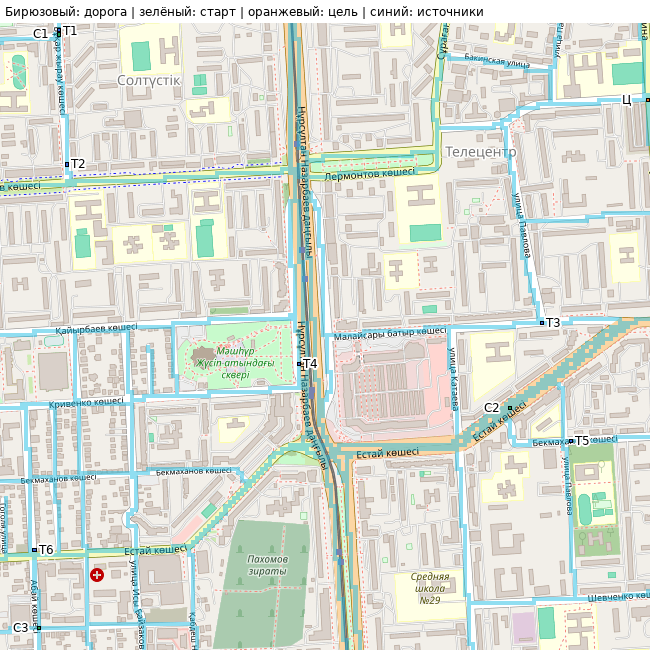
\includegraphics[width=.44\textwidth]{overlay_map.png}\hfill
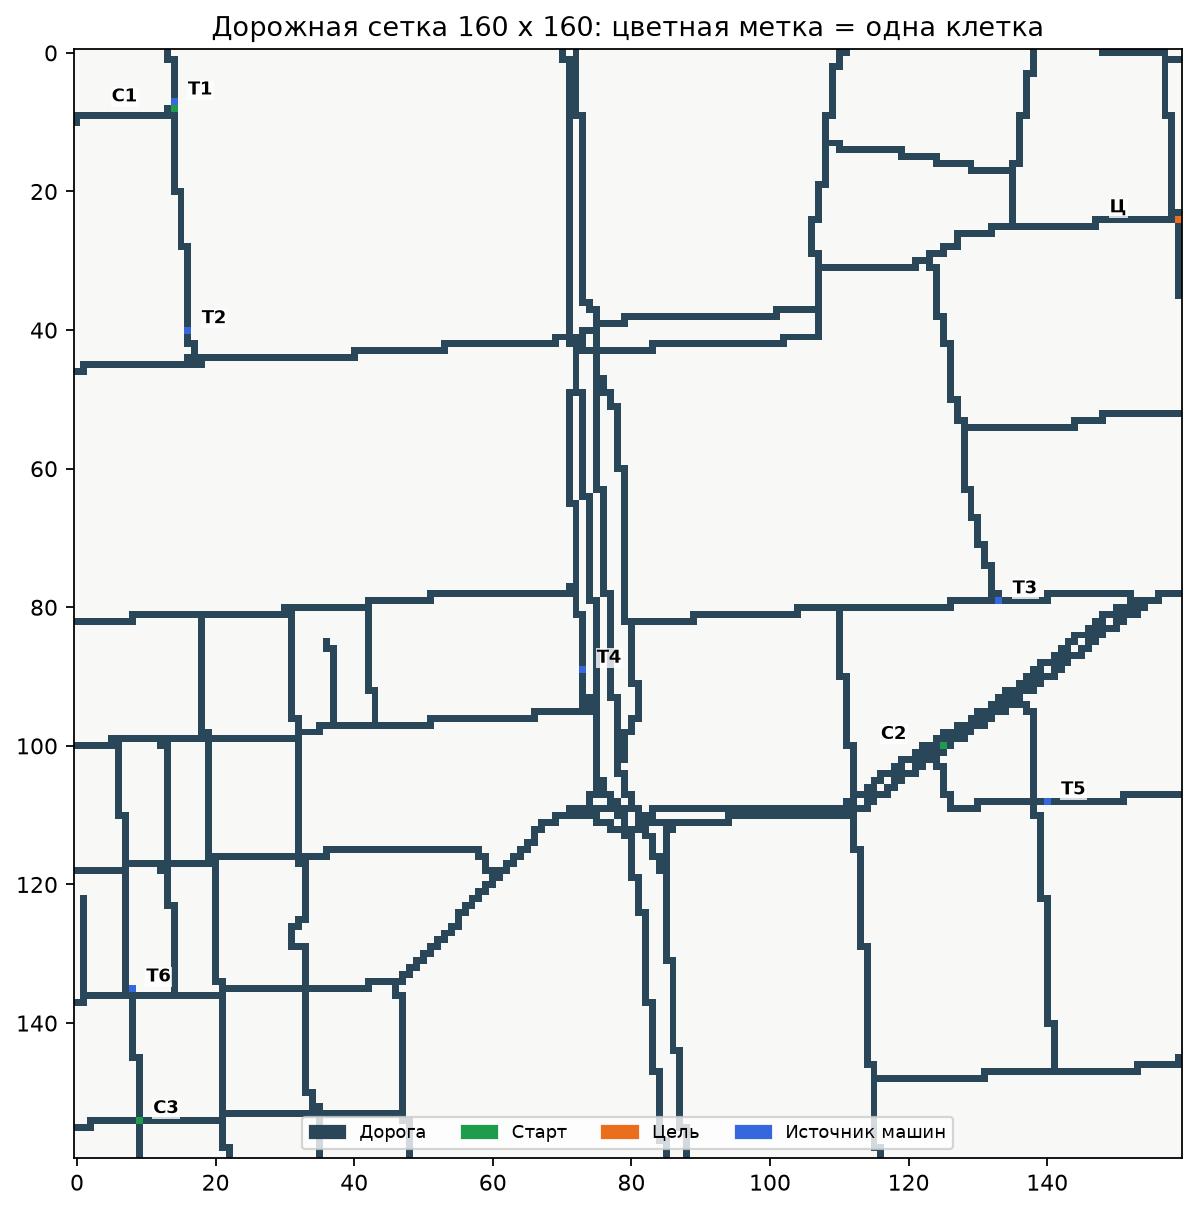
\includegraphics[width=.44\textwidth]{grid_map.png}
\caption{Исходная подложка OpenStreetMap, выбранные линии дорог, наложение клеток и итоговая сетка.}
\end{figure}

На карте расположены три старта: $(8,14)$, $(100,125)$, $(154,9)$; общая цель $(24,159)$ и шесть источников машин. Коды карты: 0 - дорога, 1 - препятствие, 2 - старт, 3 - источник, 4 - цель. Координаты показывают строку и столбец клетки.

\section{Среда и стратегии}
За шаг курьер переходит вверх, вниз, влево, вправо или останавливается. Каждый источник с вероятностью $p$ порождает машину. Время жизни машины составляет от 15 до 150 шагов. На обычном участке она с вероятностью 0,7 продолжает прежнее направление; на развилке равновероятно выбирает доступный выход. Столкновение курьера с машиной завершает поездку. В одной клетке все машины исчезают, если оказались там одновременно.

\begin{center}
\small
\begin{tabular}{|p{3.3cm}|p{5cm}|p{5.4cm}|}
\hline
Стратегия & Маршрут & Реакция на машины \\ \hline
Исследователь & Предпочитает непосещённые клетки, в том числе более далёкие от цели. & При угрозе удаляется от машин и может возвращаться по старым клеткам. \\ \hline
Нетерпеливый кратчайший & Выбирает кратчайшее расстояние до цели со штрафом за близкие машины. & Продолжает ехать; специального ожидания нет. \\ \hline
Осторожный объезд & Учитывает близость источников машин до начала движения. & Может ждать приближающуюся машину или отступить. \\ \hline
\end{tabular}
\end{center}

\section{План эксперимента}
Проверены четыре вероятности появления машины на источнике за шаг: $p=0$; $0{,}005$; $0{,}02$; $0{,}05$. Для каждого сочетания $p$, старта и стратегии выполнено 100 поездок при каждом из пяти seed. Всего получено $4\cdot3\cdot3\cdot5\cdot100=18\,000$ поездок. Лимит одной поездки - 4000 шагов; в сохранённых результатах ни одна поездка его не достигла.

Доля успешных доставок равна числу доставок, делённому на число всех поездок. Число шагов усредняется только по успешным поездкам. Поэтому оба показателя нужны вместе: короткое время у немногих выживших поездок не означает надёжную стратегию. Для диаграмм размаха каждое из пяти значений объединяет 100 поездок одного seed.

\clearpage
\section{Результаты по трём стартам}
На графиках отдельно приведены все три старта и все три стратегии. Логарифмическая шкала числа шагов позволяет показать исследователя и два более коротких маршрута на одном рисунке; подписи шкалы остаются в обычных шагах.

\subsection{Старт 1}
\begin{figure}[H]
\centering
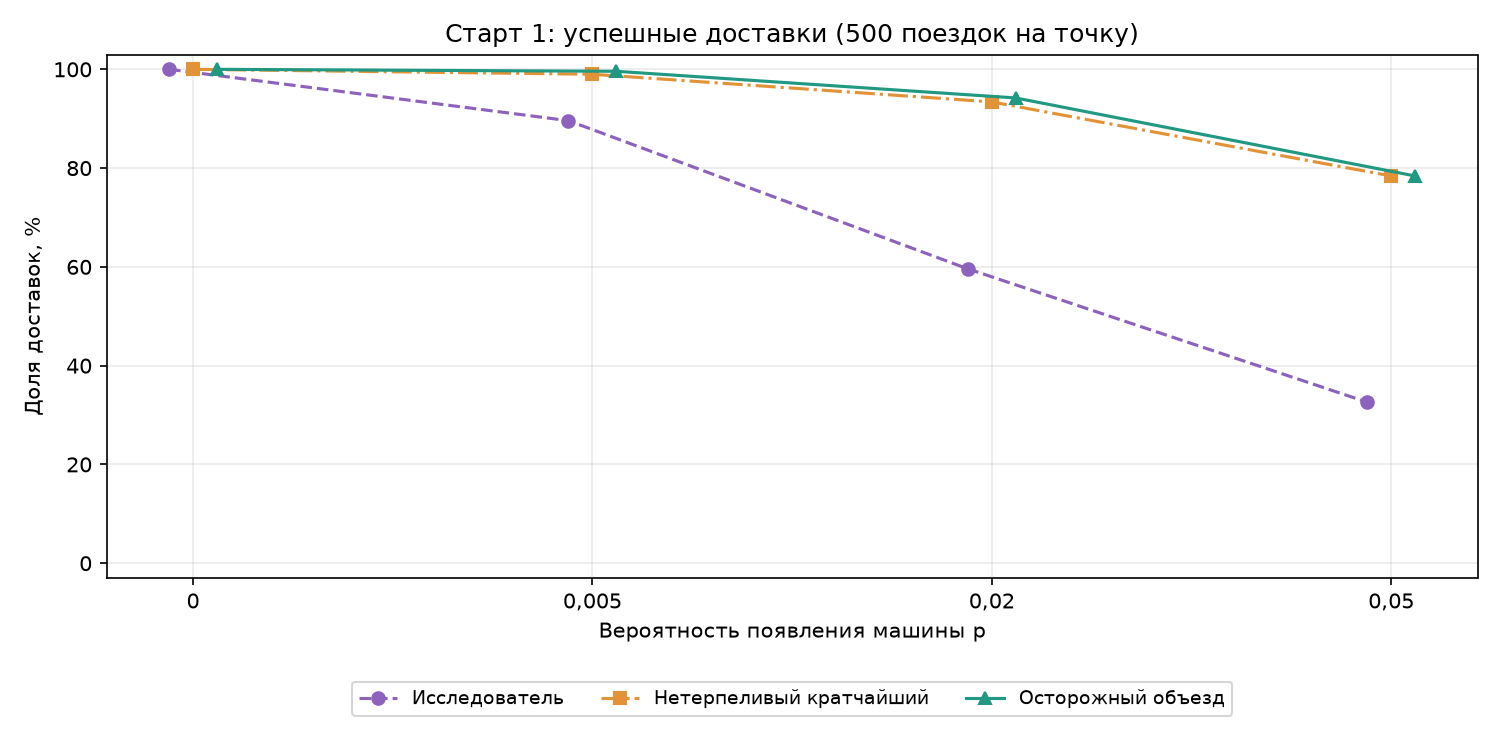
\includegraphics[width=.80\textwidth]{start_1_success_percent.png}
\caption{Доля успешных доставок со старта 1.}
\end{figure}
\begin{figure}[H]
\centering
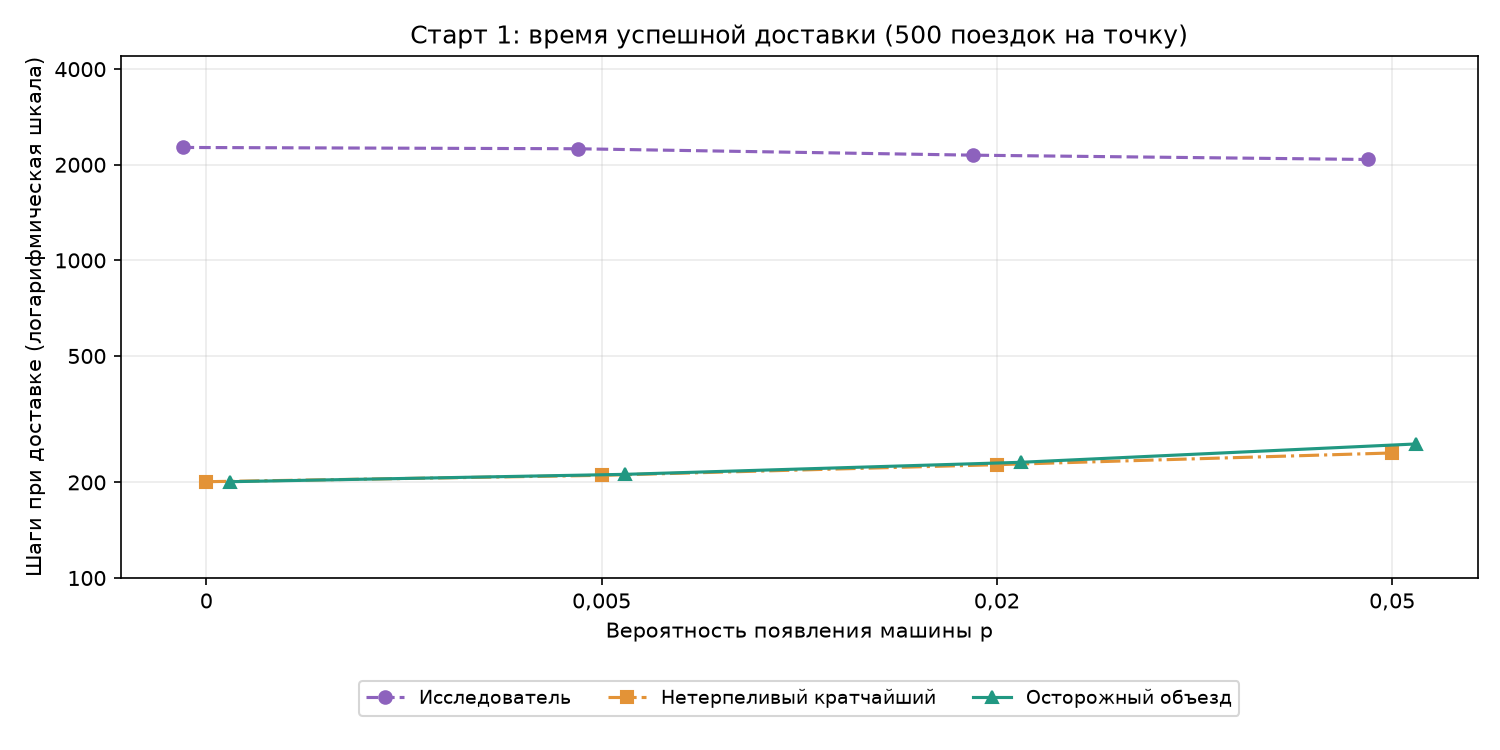
\includegraphics[width=.80\textwidth]{start_1_successful_steps.png}
\caption{Среднее число шагов успешной доставки со старта 1.}
\end{figure}
\begin{figure}[H]
\centering
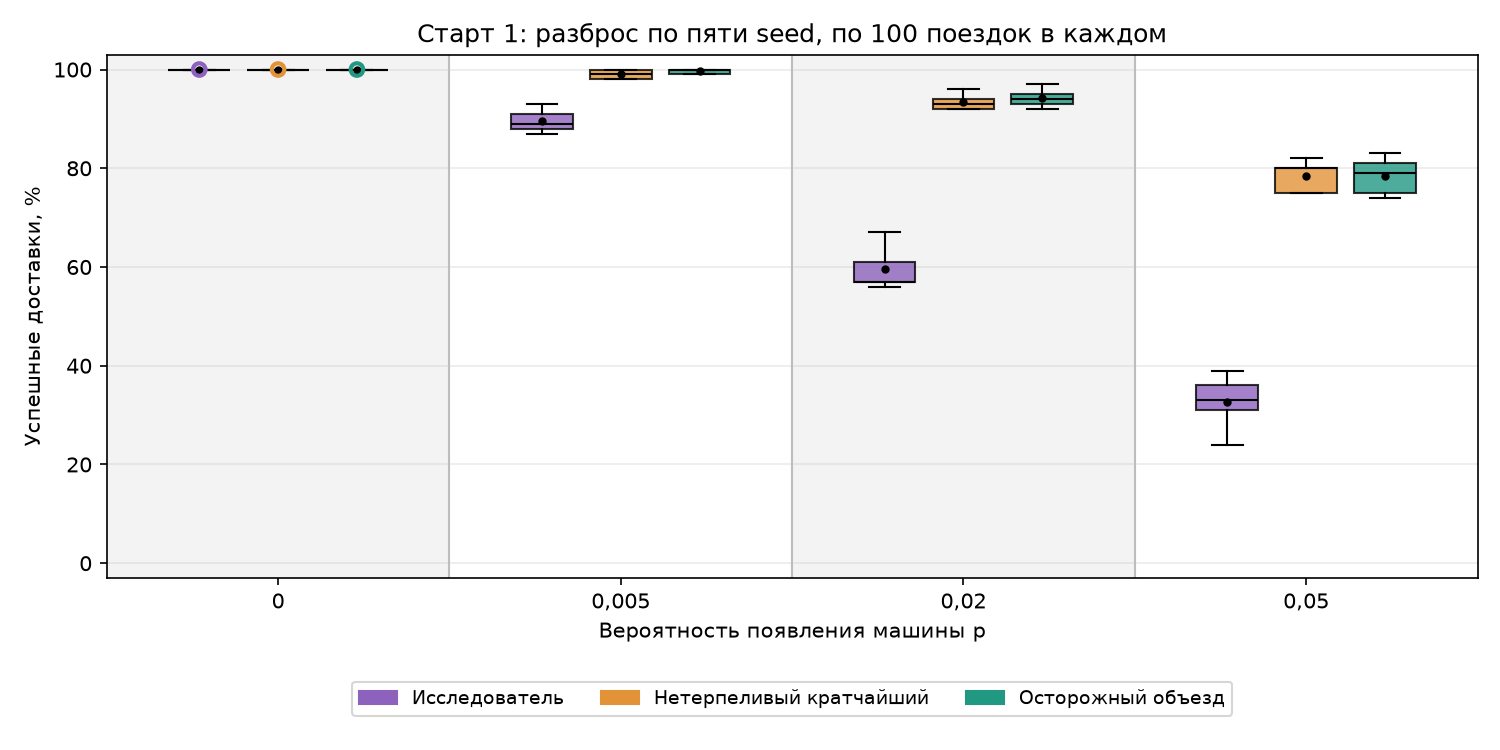
\includegraphics[width=.80\textwidth]{start_1_success_boxplot.png}
\caption{Разброс доли доставок по пяти seed со старта 1.}
\end{figure}
\begin{figure}[H]
\centering
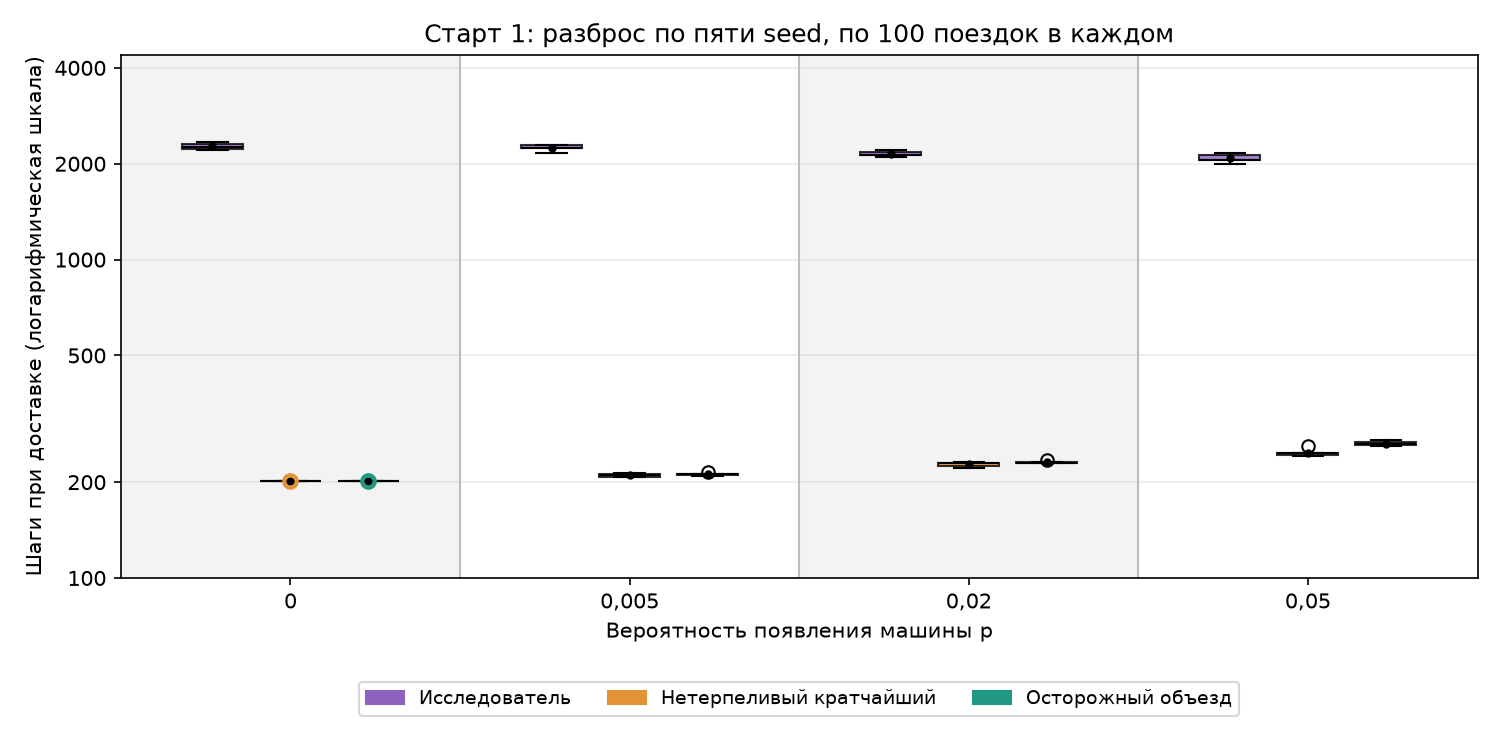
\includegraphics[width=.80\textwidth]{start_1_steps_boxplot.png}
\caption{Разброс числа шагов по пяти seed со старта 1.}
\end{figure}
\clearpage

\subsection{Старт 2}
\begin{figure}[H]
\centering
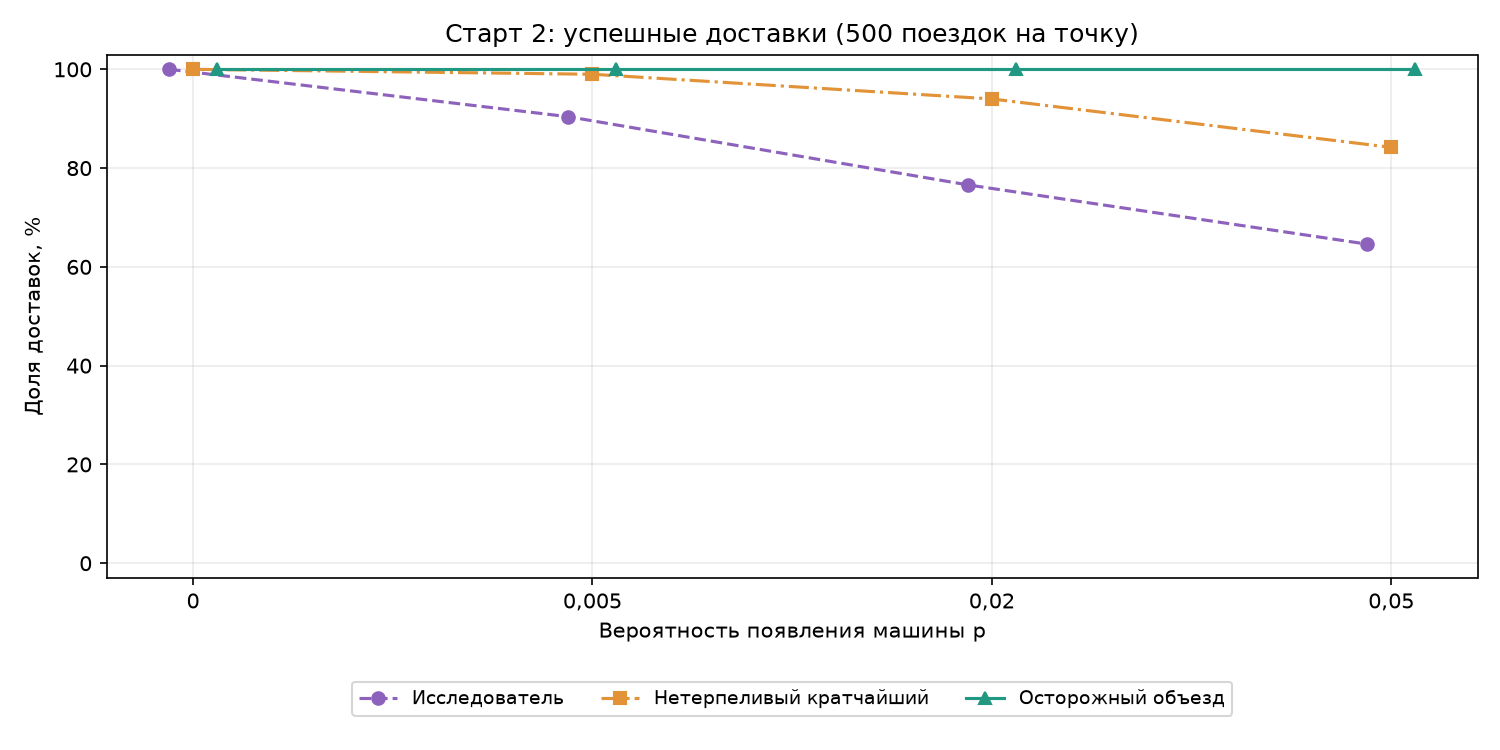
\includegraphics[width=.80\textwidth]{start_2_success_percent.png}
\caption{Доля успешных доставок со старта 2.}
\end{figure}
\begin{figure}[H]
\centering
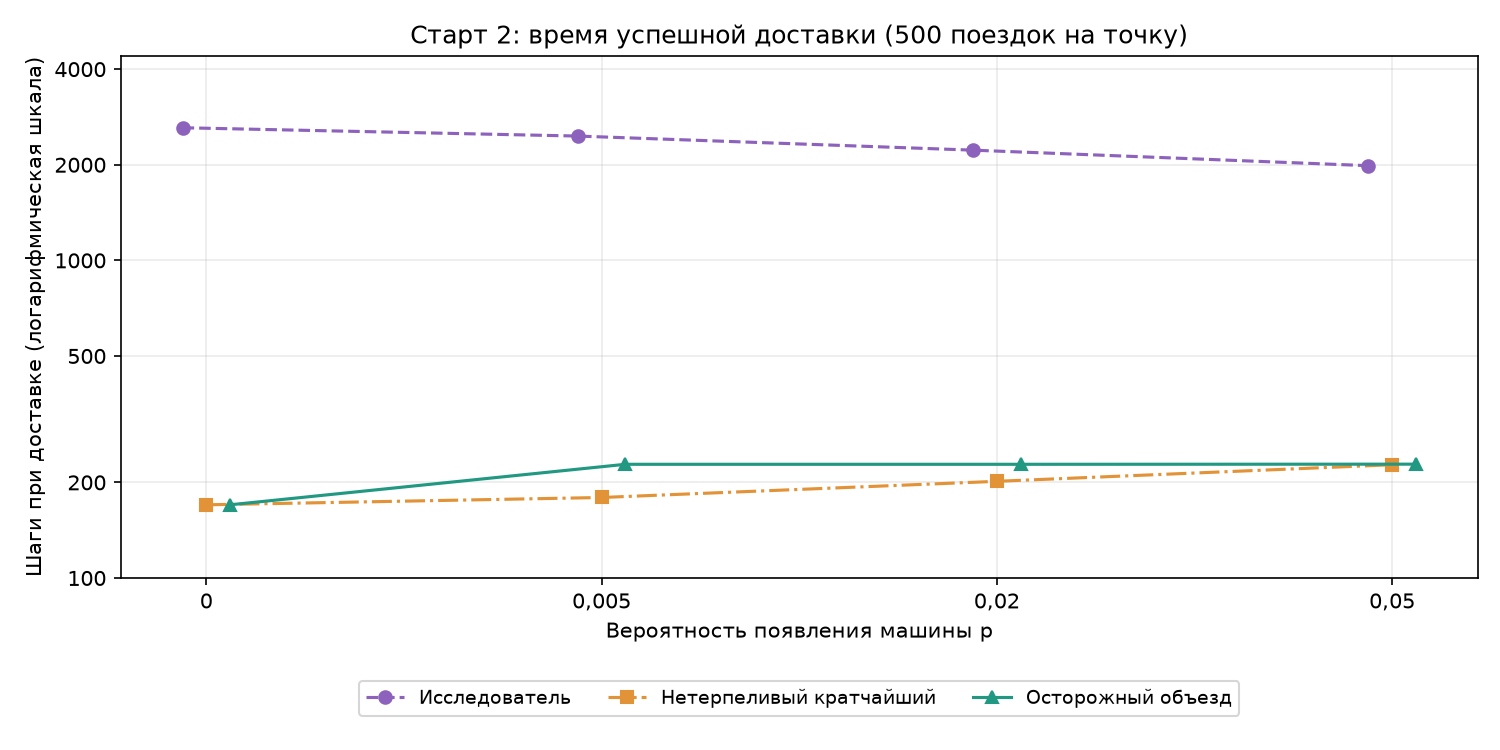
\includegraphics[width=.80\textwidth]{start_2_successful_steps.png}
\caption{Среднее число шагов успешной доставки со старта 2.}
\end{figure}
\begin{figure}[H]
\centering
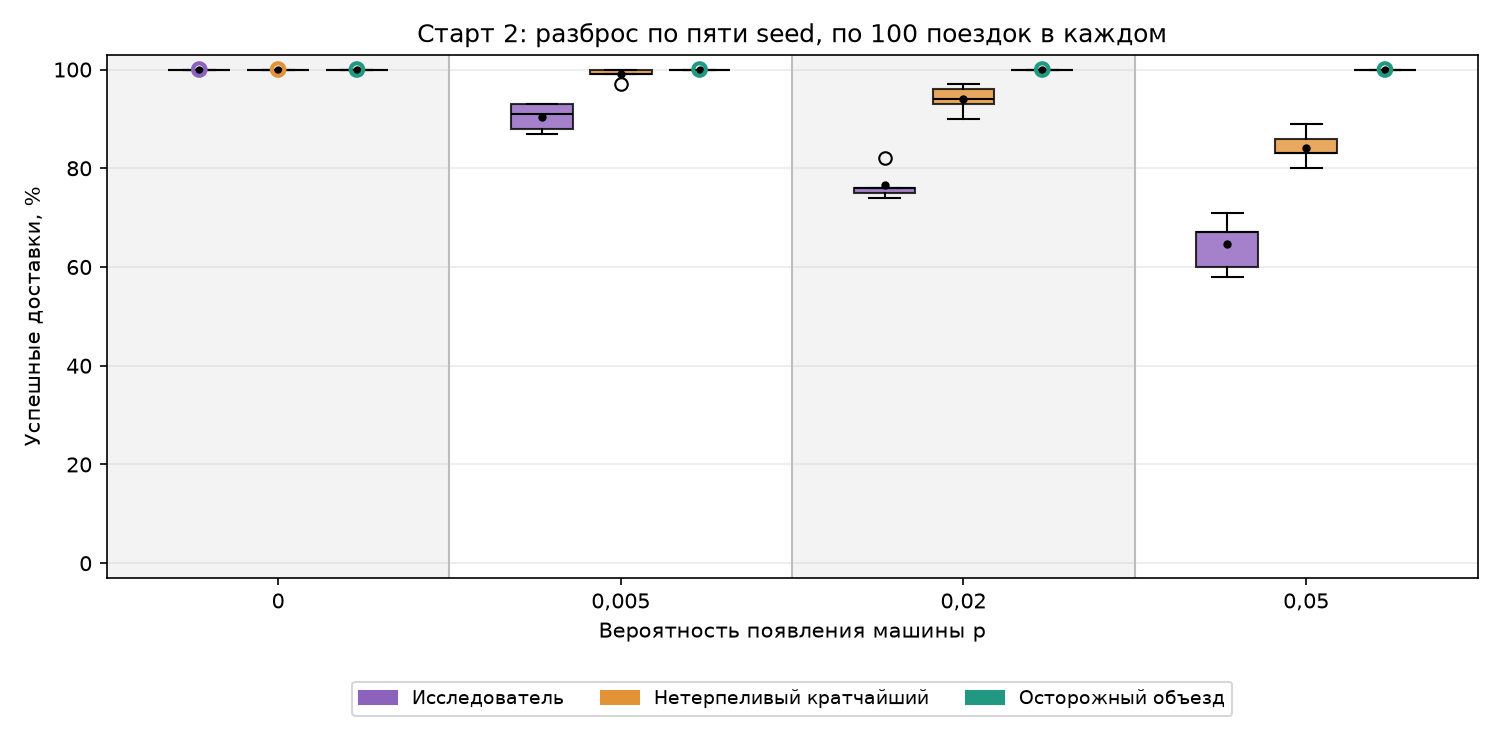
\includegraphics[width=.80\textwidth]{start_2_success_boxplot.png}
\caption{Разброс доли доставок по пяти seed со старта 2.}
\end{figure}
\begin{figure}[H]
\centering
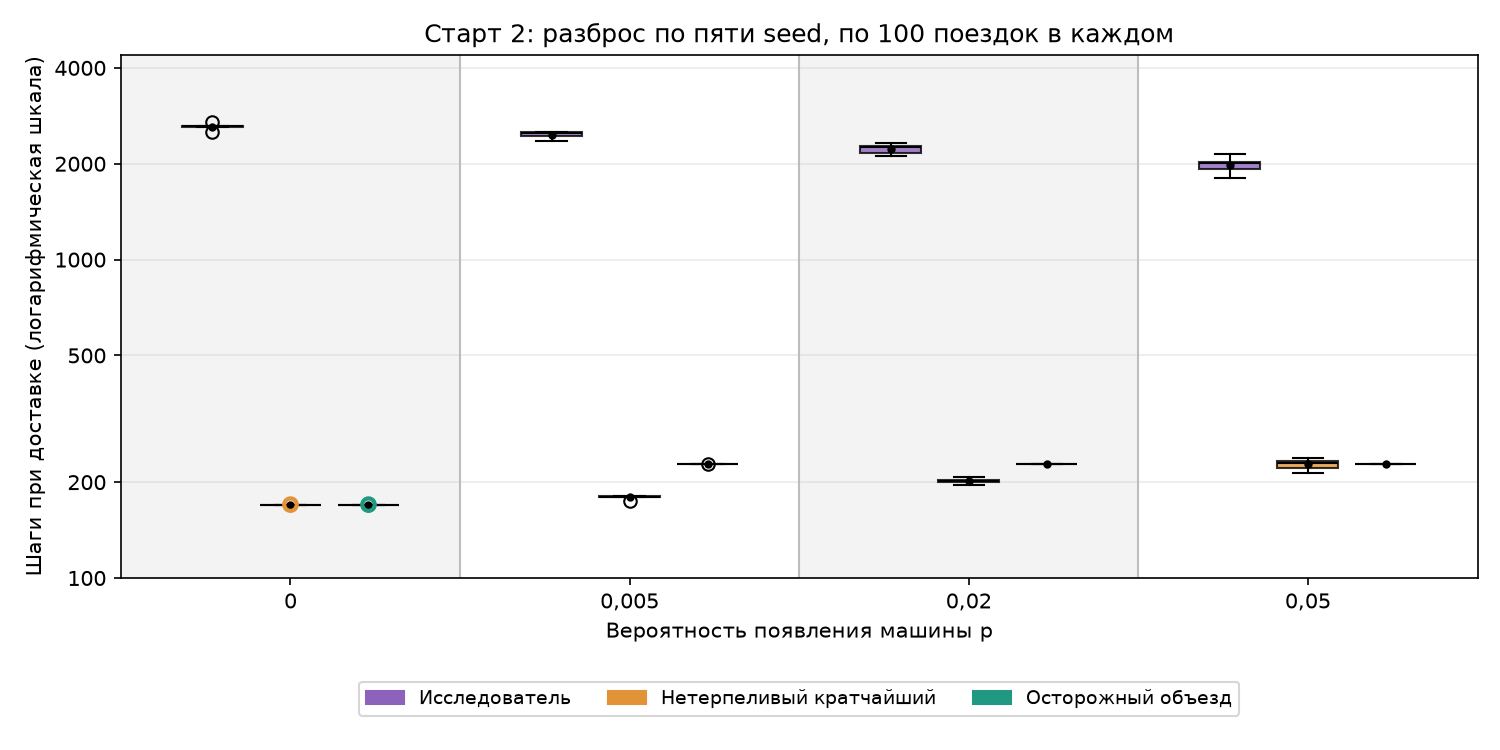
\includegraphics[width=.80\textwidth]{start_2_steps_boxplot.png}
\caption{Разброс числа шагов по пяти seed со старта 2.}
\end{figure}
\clearpage

\subsection{Старт 3}
\begin{figure}[H]
\centering
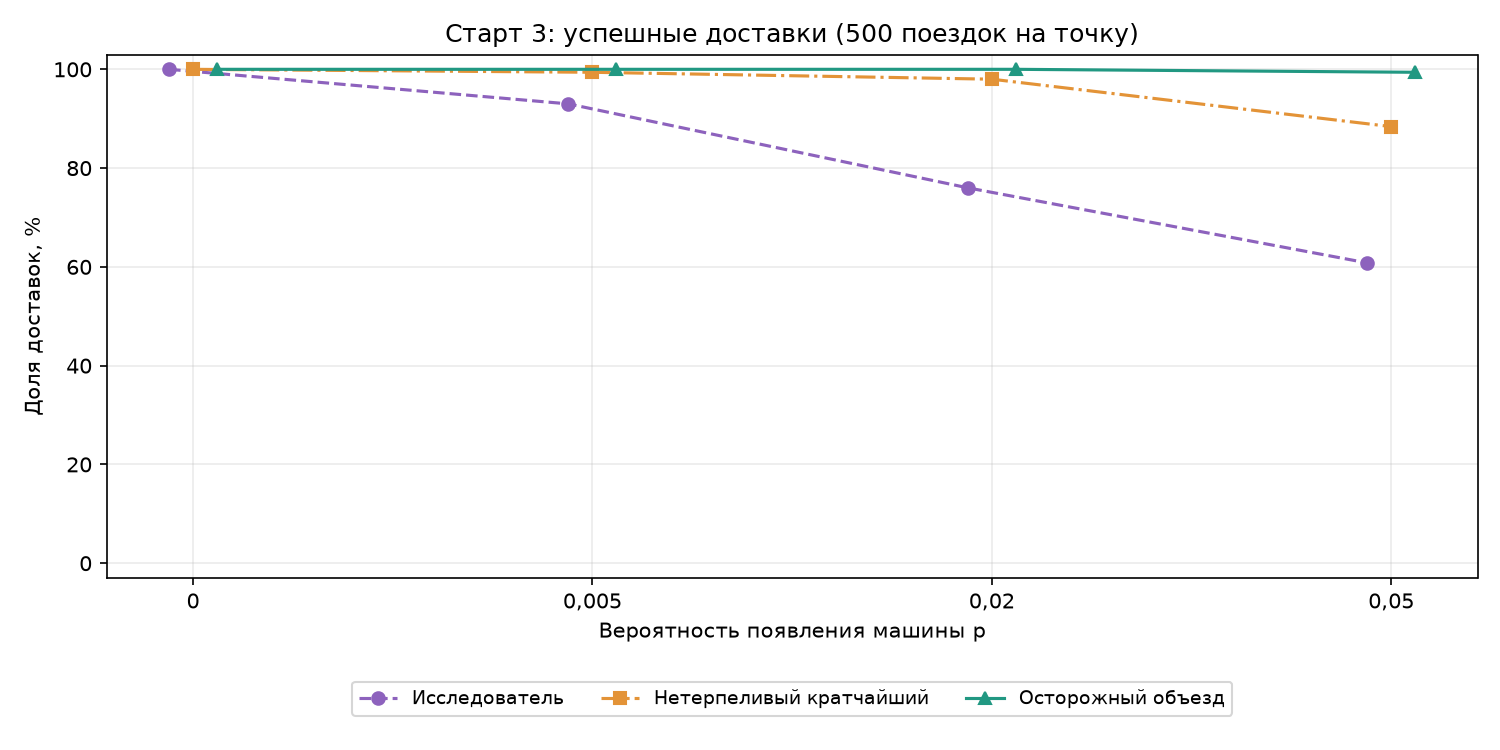
\includegraphics[width=.80\textwidth]{start_3_success_percent.png}
\caption{Доля успешных доставок со старта 3.}
\end{figure}
\begin{figure}[H]
\centering
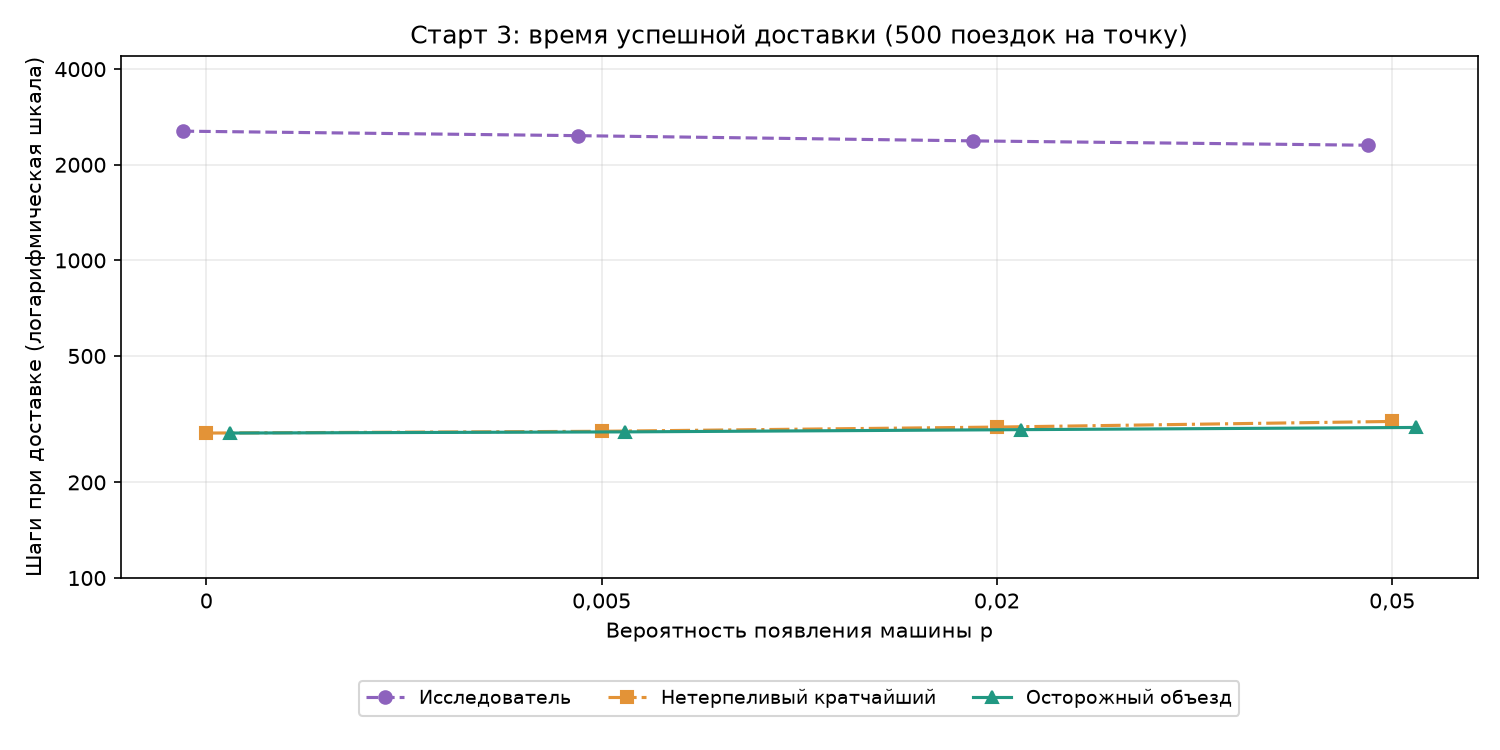
\includegraphics[width=.80\textwidth]{start_3_successful_steps.png}
\caption{Среднее число шагов успешной доставки со старта 3.}
\end{figure}
\begin{figure}[H]
\centering
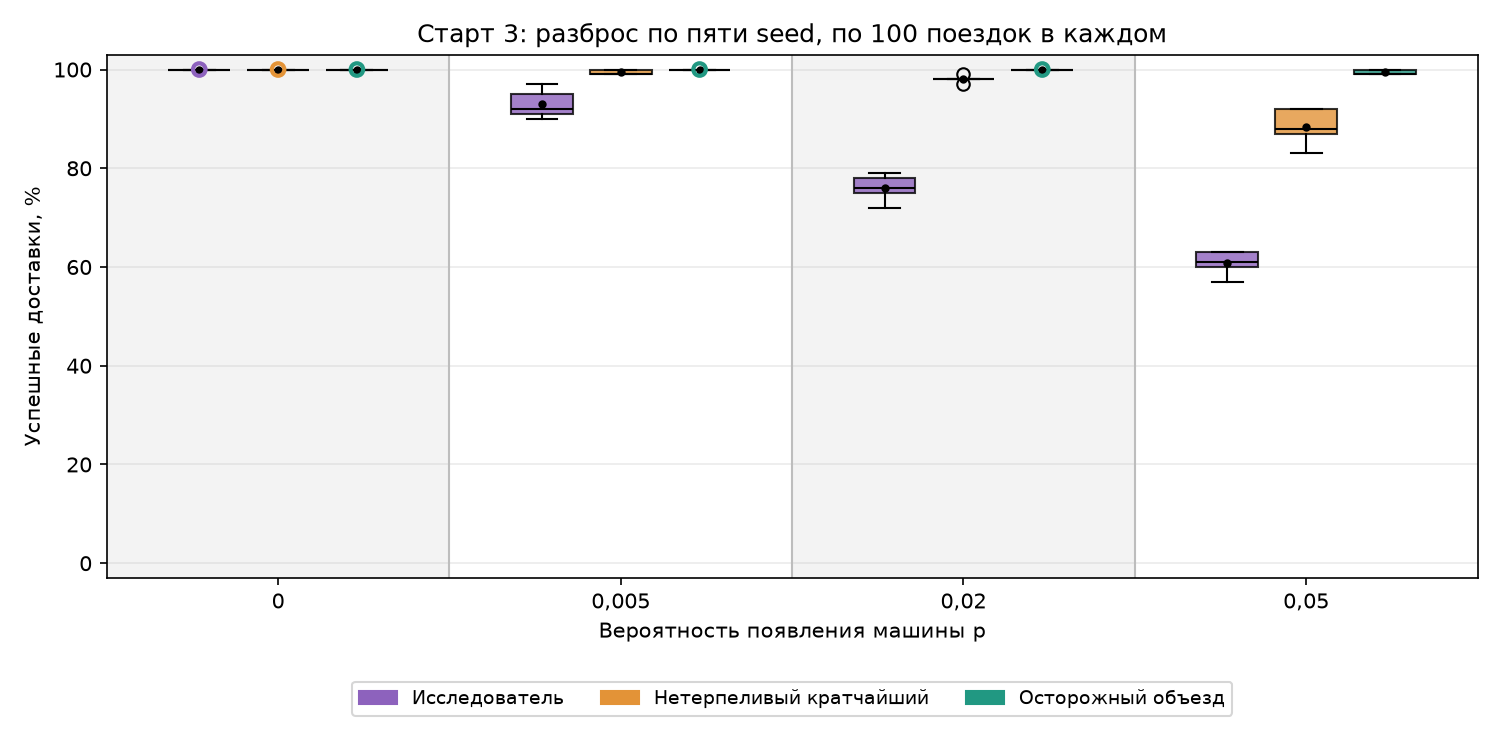
\includegraphics[width=.80\textwidth]{start_3_success_boxplot.png}
\caption{Разброс доли доставок по пяти seed со старта 3.}
\end{figure}
\begin{figure}[H]
\centering
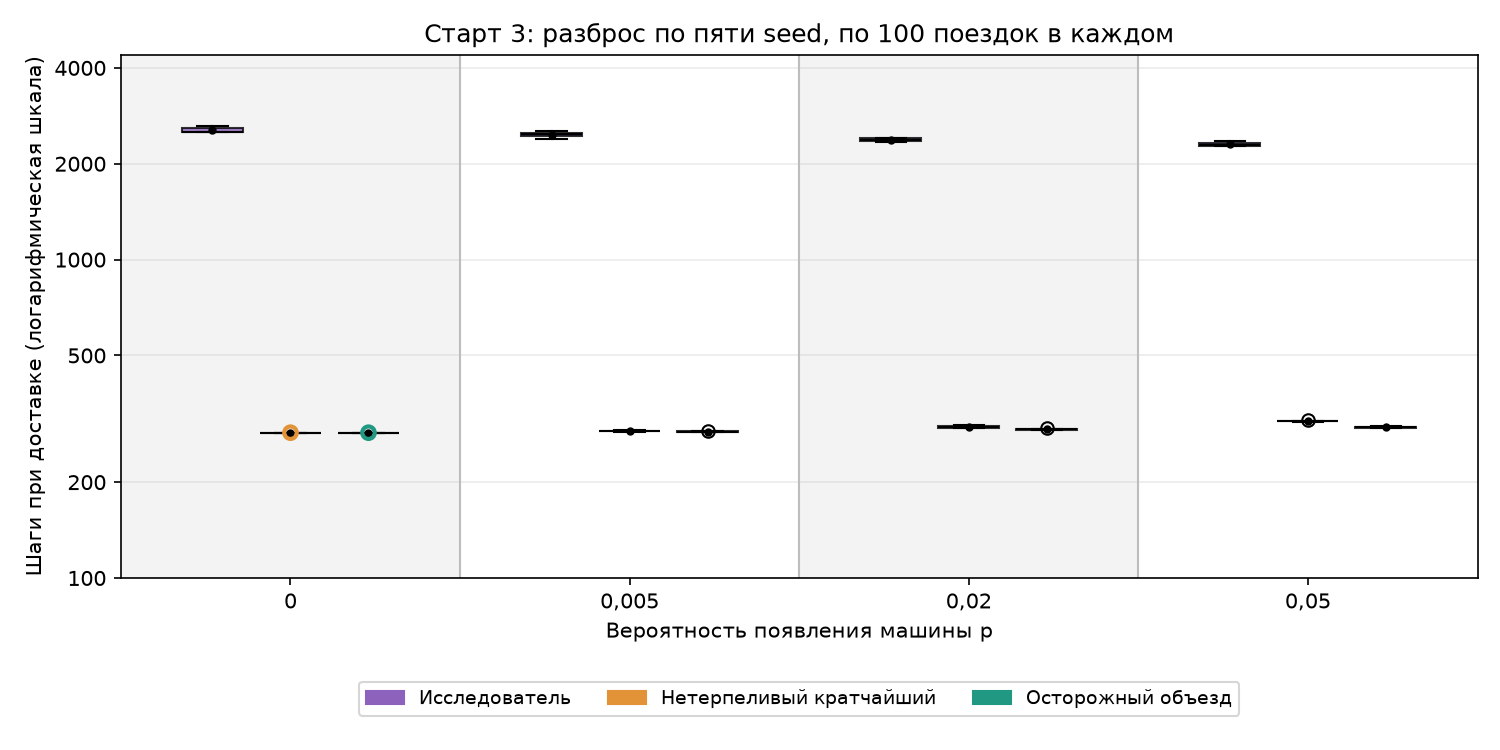
\includegraphics[width=.80\textwidth]{start_3_steps_boxplot.png}
\caption{Разброс числа шагов по пяти seed со старта 3.}
\end{figure}

\section{Таблицы для всех вероятностей появления машин}
Каждая строка основана на 500 поездках: 100 при каждом из пяти seed. Среднее число шагов рассчитано только для успешных доставок.

\begin{table}[H]
\centering
\footnotesize
\caption{Подробные результаты при $p=0$.}
\begin{tabular}{|c|p{4.6cm}|c|c|c|c|}
\hline
Старт & Стратегия & Доставки & Поездки & Успех, \% & Шаги \\ \hline
1 & Исследователь & 500 & 500 & 100,0 & 2267,37 \\ \hline
1 & Нетерпеливый кратчайший & 500 & 500 & 100,0 & 201,00 \\ \hline
1 & Осторожный объезд & 500 & 500 & 100,0 & 201,00 \\ \hline
2 & Исследователь & 500 & 500 & 100,0 & 2615,54 \\ \hline
2 & Нетерпеливый кратчайший & 500 & 500 & 100,0 & 170,00 \\ \hline
2 & Осторожный объезд & 500 & 500 & 100,0 & 170,00 \\ \hline
3 & Исследователь & 500 & 500 & 100,0 & 2551,75 \\ \hline
3 & Нетерпеливый кратчайший & 500 & 500 & 100,0 & 286,00 \\ \hline
3 & Осторожный объезд & 500 & 500 & 100,0 & 286,00 \\ \hline
\end{tabular}
\end{table}

\begin{table}[H]
\centering
\footnotesize
\caption{Подробные результаты при $p=0,005$.}
\begin{tabular}{|c|p{4.6cm}|c|c|c|c|}
\hline
Старт & Стратегия & Доставки & Поездки & Успех, \% & Шаги \\ \hline
1 & Исследователь & 448 & 500 & 89,6 & 2245,97 \\ \hline
1 & Нетерпеливый кратчайший & 495 & 500 & 99,0 & 210,50 \\ \hline
1 & Осторожный объезд & 498 & 500 & 99,6 & 212,03 \\ \hline
2 & Исследователь & 452 & 500 & 90,4 & 2462,59 \\ \hline
2 & Нетерпеливый кратчайший & 495 & 500 & 99,0 & 179,25 \\ \hline
2 & Осторожный объезд & 500 & 500 & 100,0 & 228,03 \\ \hline
3 & Исследователь & 465 & 500 & 93,0 & 2469,97 \\ \hline
3 & Нетерпеливый кратчайший & 497 & 500 & 99,4 & 289,67 \\ \hline
3 & Осторожный объезд & 500 & 500 & 100,0 & 288,44 \\ \hline
\end{tabular}
\end{table}

\begin{table}[H]
\centering
\footnotesize
\caption{Подробные результаты при $p=0,02$.}
\begin{tabular}{|c|p{4.6cm}|c|c|c|c|}
\hline
Старт & Стратегия & Доставки & Поездки & Успех, \% & Шаги \\ \hline
1 & Исследователь & 298 & 500 & 59,6 & 2143,99 \\ \hline
1 & Нетерпеливый кратчайший & 467 & 500 & 93,4 & 227,37 \\ \hline
1 & Осторожный объезд & 471 & 500 & 94,2 & 231,35 \\ \hline
2 & Исследователь & 383 & 500 & 76,6 & 2223,45 \\ \hline
2 & Нетерпеливый кратчайший & 470 & 500 & 94,0 & 201,56 \\ \hline
2 & Осторожный объезд & 500 & 500 & 100,0 & 228,03 \\ \hline
3 & Исследователь & 380 & 500 & 76,0 & 2378,03 \\ \hline
3 & Нетерпеливый кратчайший & 490 & 500 & 98,0 & 298,66 \\ \hline
3 & Осторожный объезд & 500 & 500 & 100,0 & 293,15 \\ \hline
\end{tabular}
\end{table}

\begin{table}[H]
\centering
\footnotesize
\caption{Подробные результаты при $p=0,05$.}
\begin{tabular}{|c|p{4.6cm}|c|c|c|c|}
\hline
Старт & Стратегия & Доставки & Поездки & Успех, \% & Шаги \\ \hline
1 & Исследователь & 163 & 500 & 32,6 & 2077,95 \\ \hline
1 & Нетерпеливый кратчайший & 392 & 500 & 78,4 & 247,57 \\ \hline
1 & Осторожный объезд & 392 & 500 & 78,4 & 264,26 \\ \hline
2 & Исследователь & 323 & 500 & 64,6 & 1986,80 \\ \hline
2 & Нетерпеливый кратчайший & 421 & 500 & 84,2 & 227,31 \\ \hline
2 & Осторожный объезд & 500 & 500 & 100,0 & 228,26 \\ \hline
3 & Исследователь & 304 & 500 & 60,8 & 2303,88 \\ \hline
3 & Нетерпеливый кратчайший & 442 & 500 & 88,4 & 311,13 \\ \hline
3 & Осторожный объезд & 497 & 500 & 99,4 & 297,84 \\ \hline
\end{tabular}
\end{table}

\clearpage
\section{Сравнение отдельных маршрутов}
Карты ниже показывают по одному отдельному эпизоду на каждый старт. Для трёх стратегий внутри одного старта использованы одинаковые условия трафика. Чёрный пунктир на изображениях обозначает кратчайший путь без машин; подпись над картой указывает исход и число шагов. Эти примеры иллюстрируют поведение, а выводы о надёжности основаны на массовом эксперименте.

\subsection{Старт 1, эпизод 211}
\begin{figure}[H]
\centering
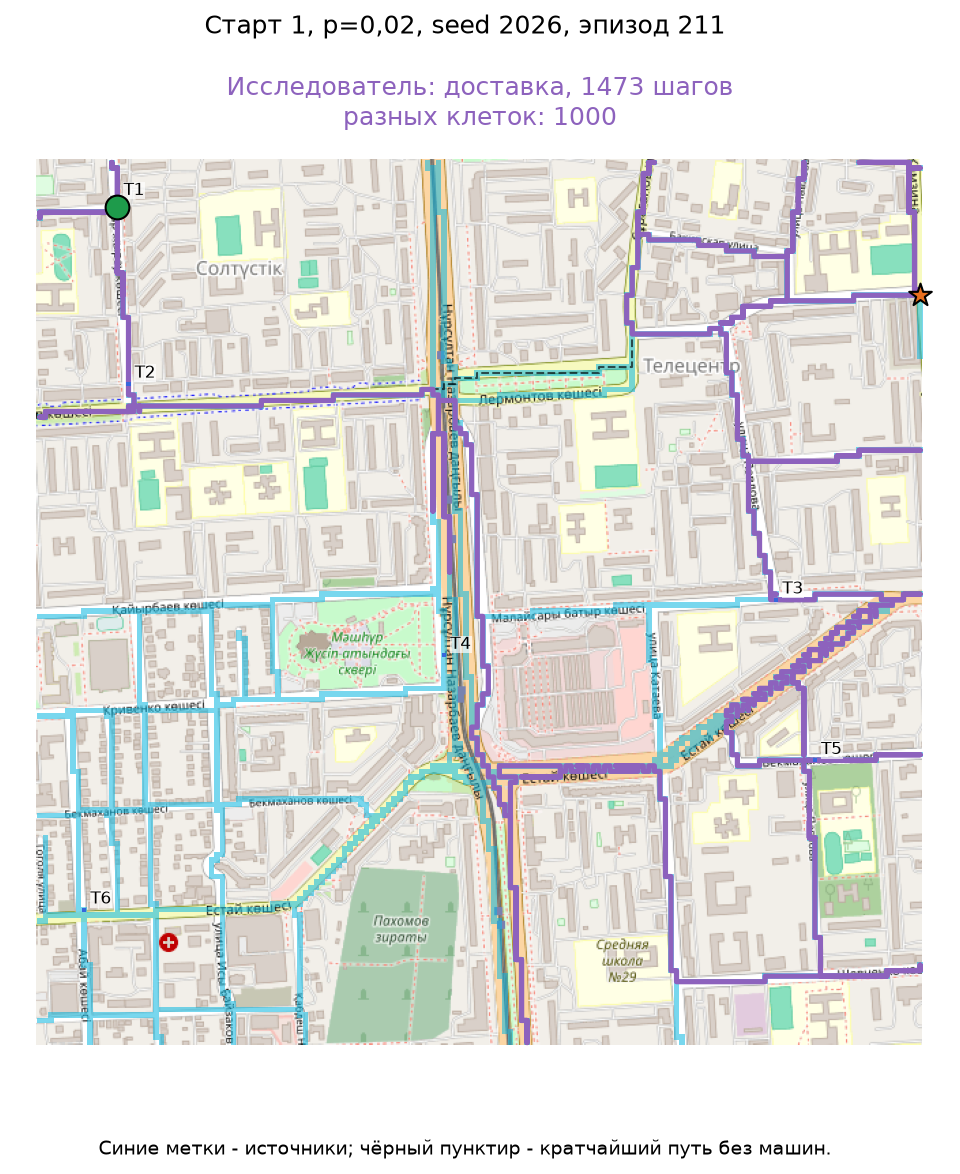
\includegraphics[height=.70\textheight]{start_1_explorer_route.png}
\caption{Исследователь: маршрут со старта 1.}
\end{figure}
\begin{figure}[H]
\centering
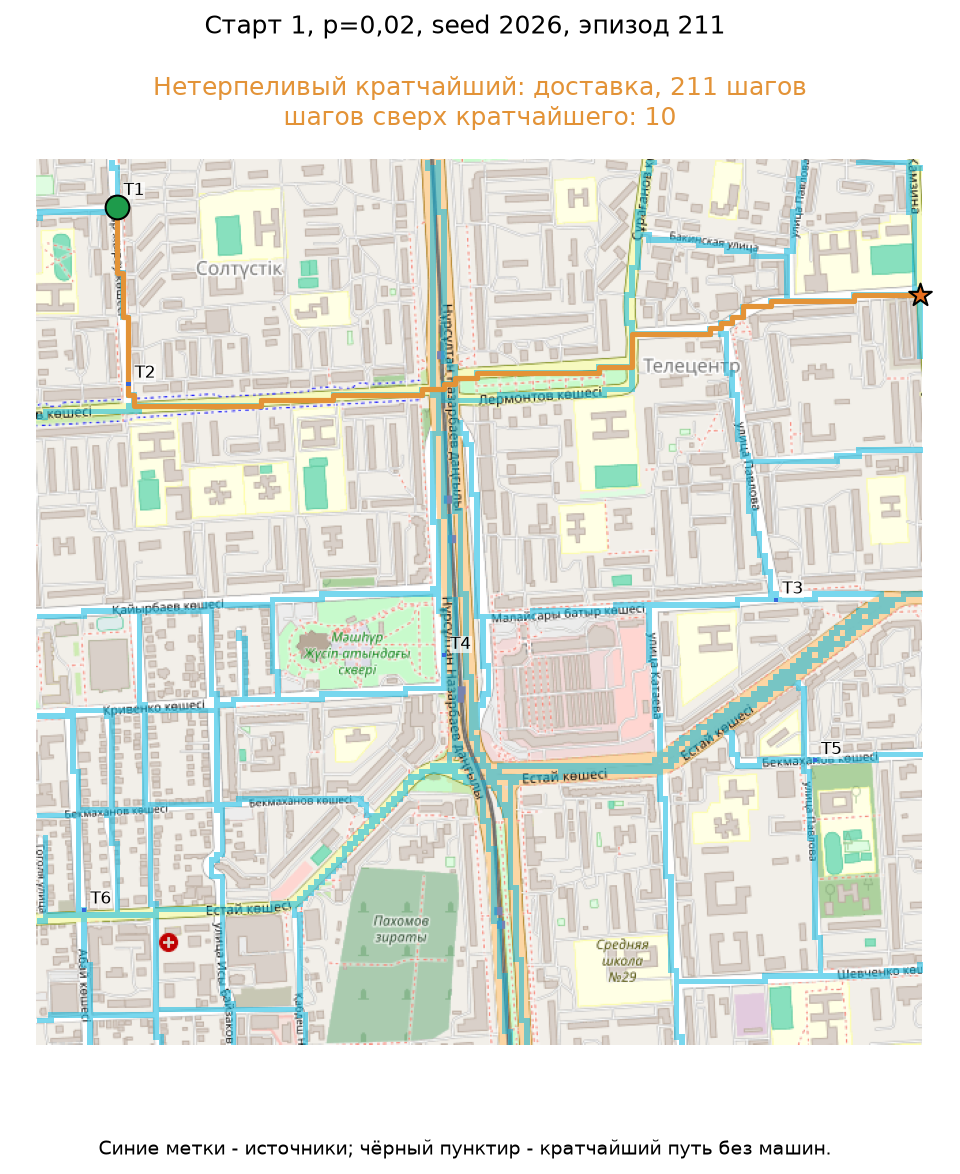
\includegraphics[height=.70\textheight]{start_1_shortest_path_route.png}
\caption{Нетерпеливый кратчайший: маршрут со старта 1.}
\end{figure}
\begin{figure}[H]
\centering
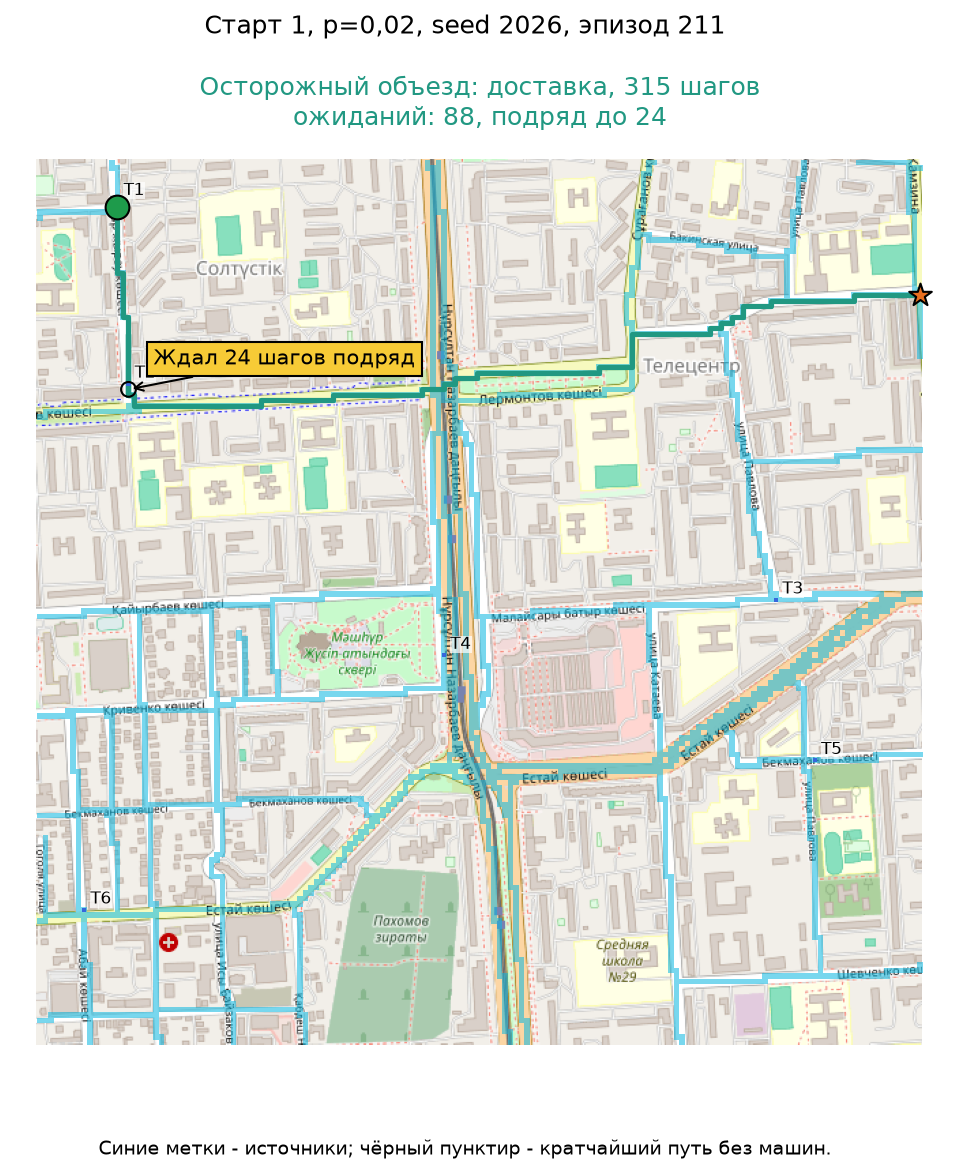
\includegraphics[height=.70\textheight]{start_1_traffic_aware_route.png}
\caption{Осторожный объезд: маршрут со старта 1.}
\end{figure}
\clearpage

\subsection{Старт 2, эпизод 97}
\begin{figure}[H]
\centering
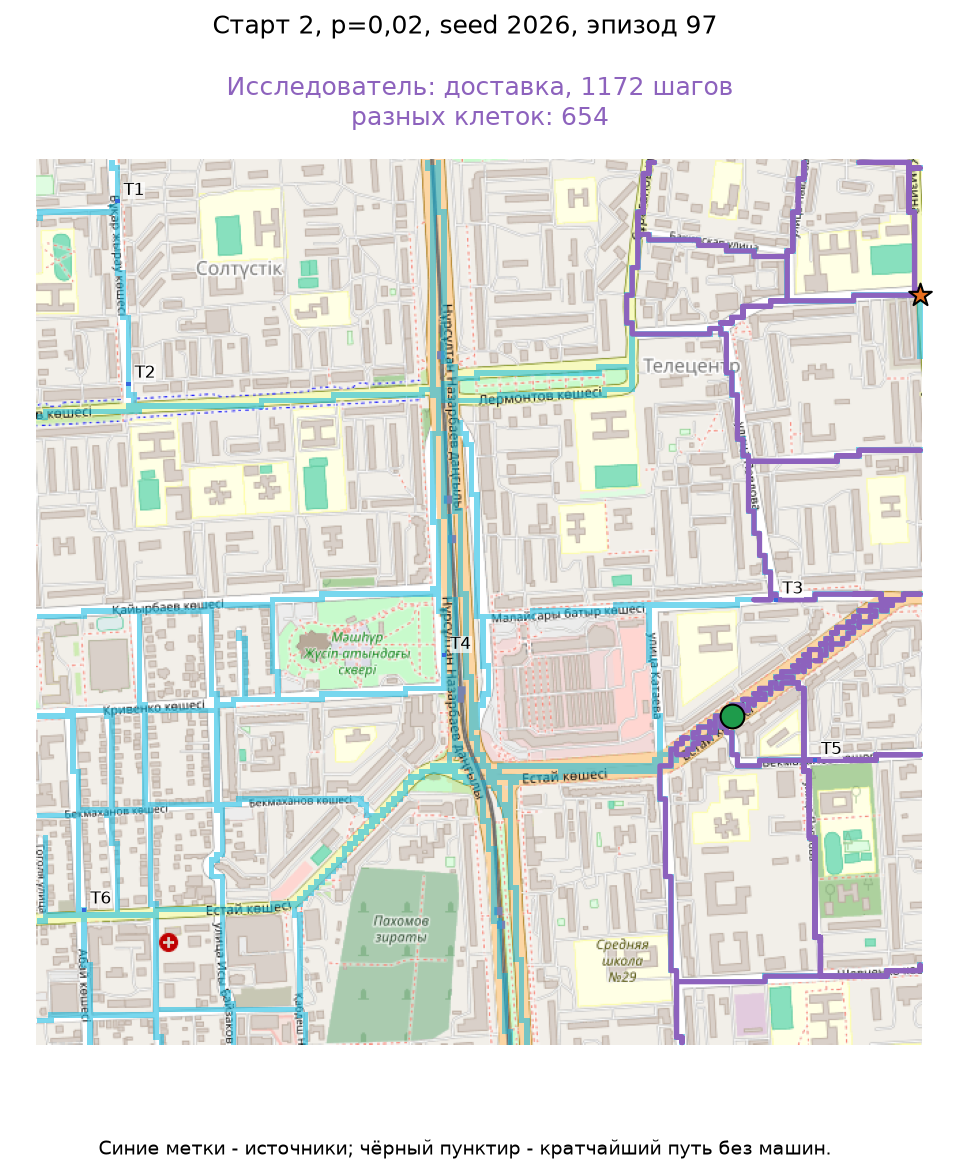
\includegraphics[height=.70\textheight]{start_2_explorer_route.png}
\caption{Исследователь: маршрут со старта 2.}
\end{figure}
\begin{figure}[H]
\centering
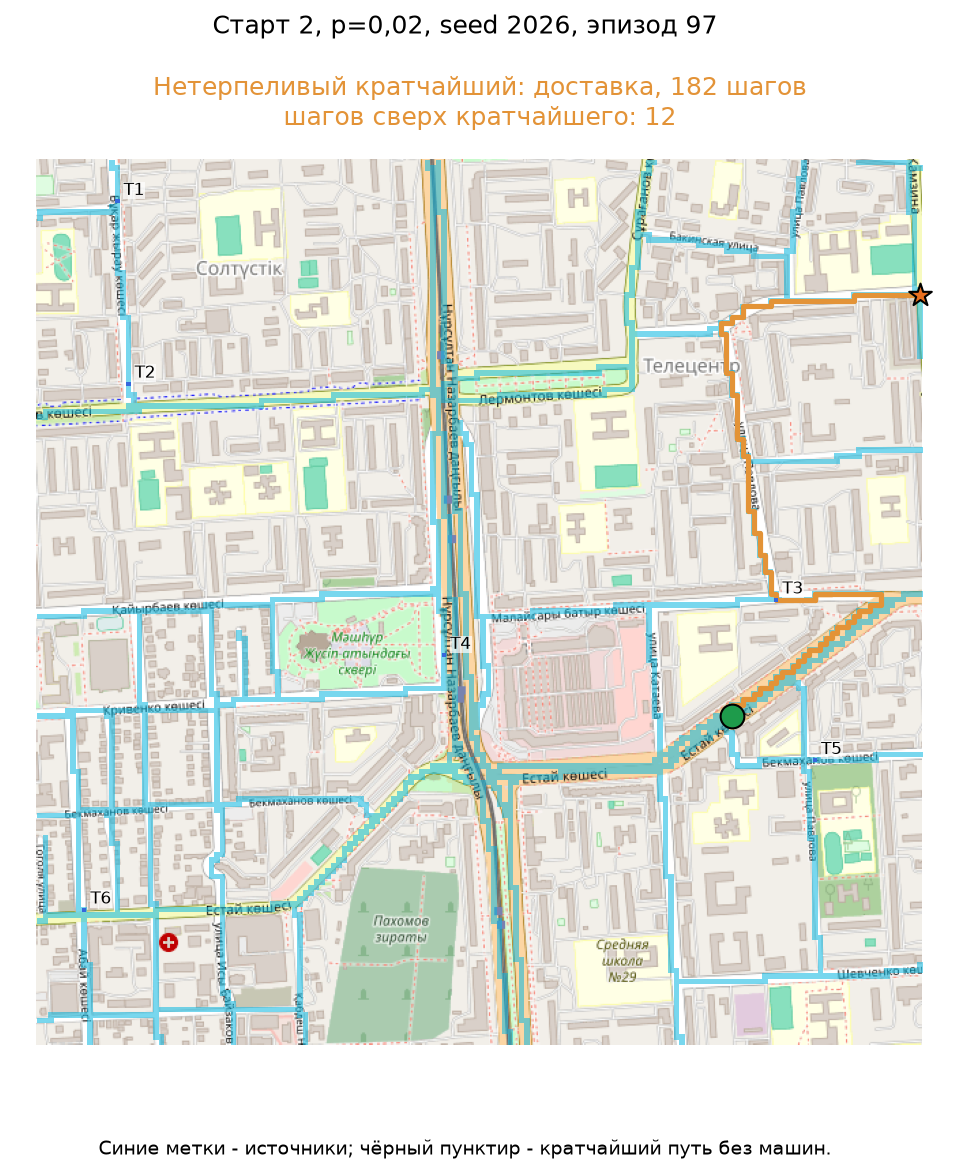
\includegraphics[height=.70\textheight]{start_2_shortest_path_route.png}
\caption{Нетерпеливый кратчайший: маршрут со старта 2.}
\end{figure}
\begin{figure}[H]
\centering
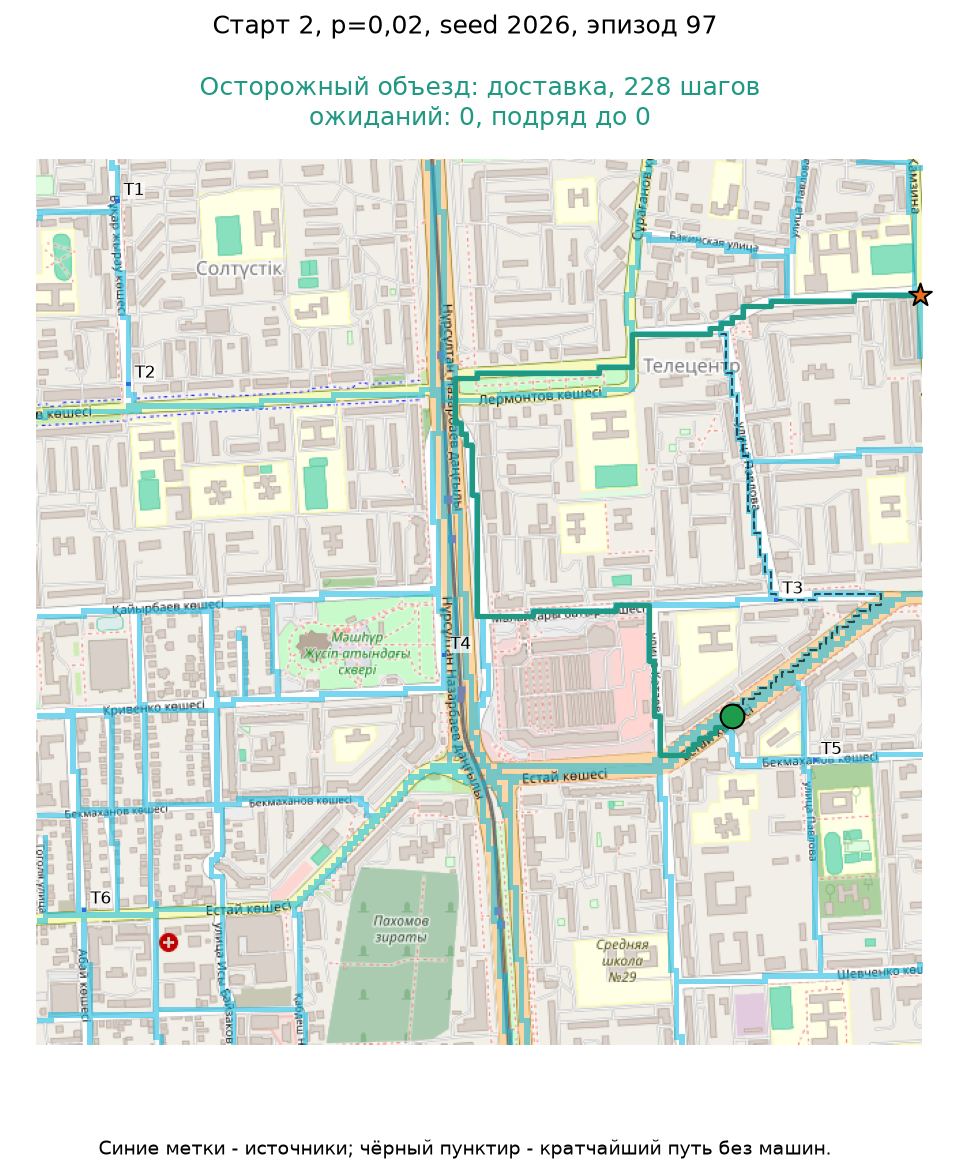
\includegraphics[height=.70\textheight]{start_2_traffic_aware_route.png}
\caption{Осторожный объезд: маршрут со старта 2.}
\end{figure}
\clearpage

\subsection{Старт 3, эпизод 47}
\begin{figure}[H]
\centering
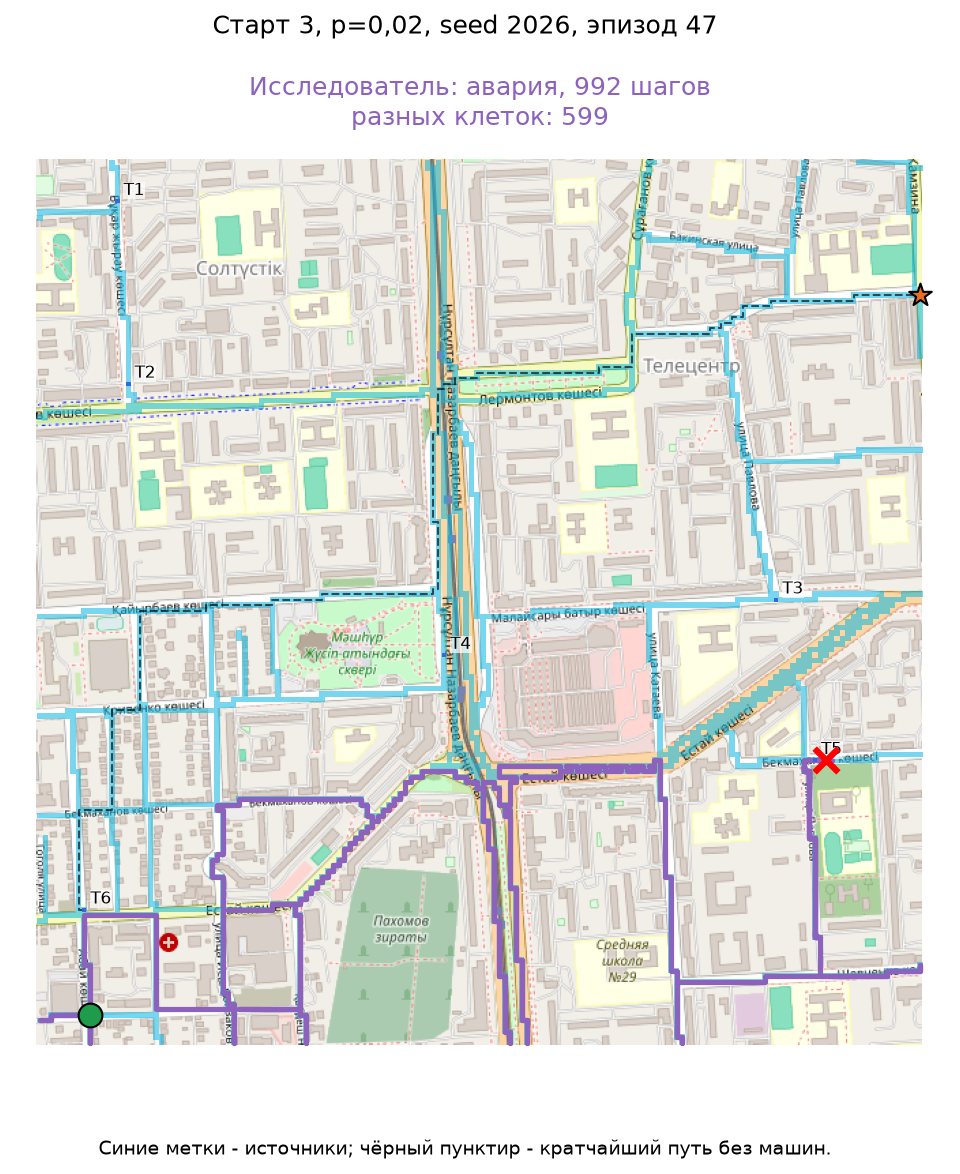
\includegraphics[height=.70\textheight]{start_3_explorer_route.png}
\caption{Исследователь: маршрут со старта 3.}
\end{figure}
\begin{figure}[H]
\centering
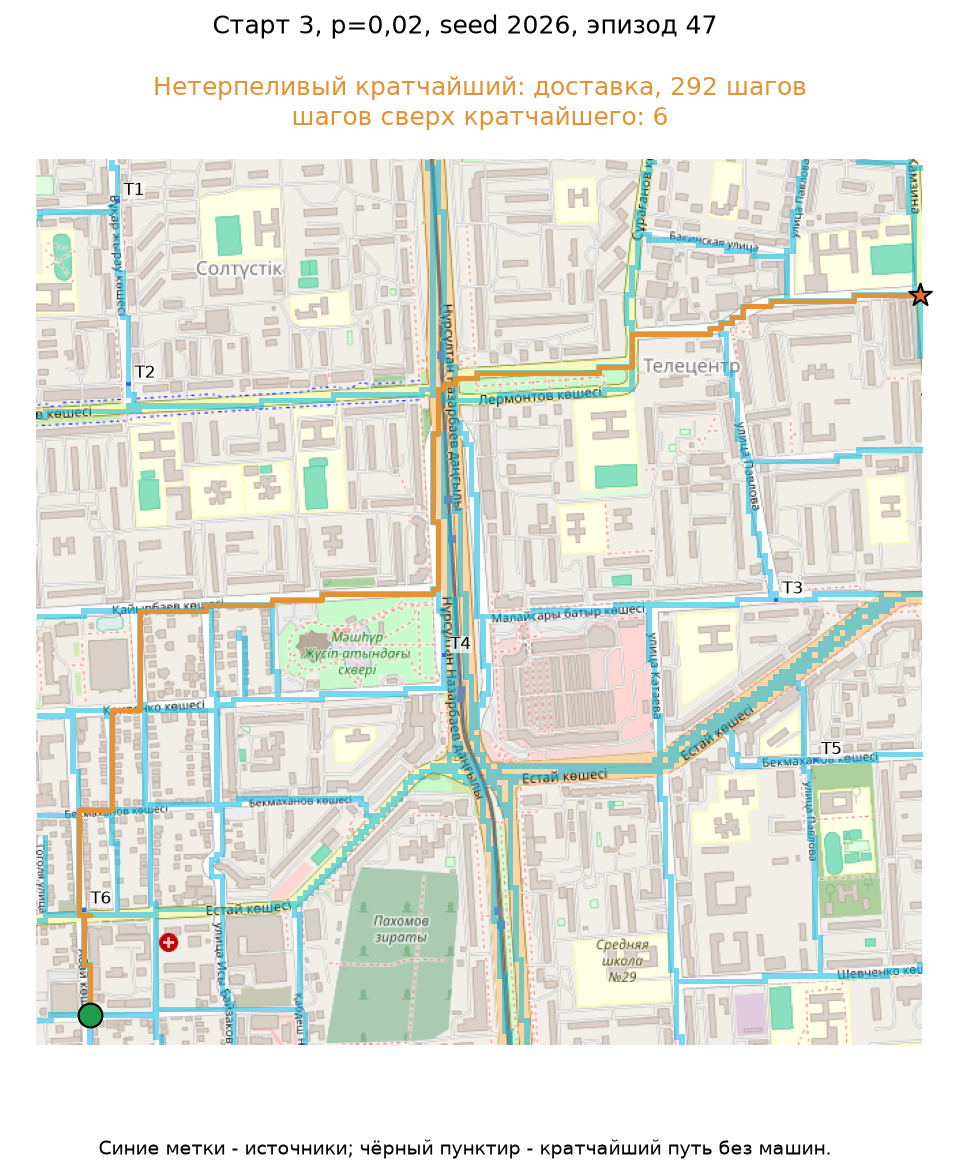
\includegraphics[height=.70\textheight]{start_3_shortest_path_route.png}
\caption{Нетерпеливый кратчайший: маршрут со старта 3.}
\end{figure}
\begin{figure}[H]
\centering
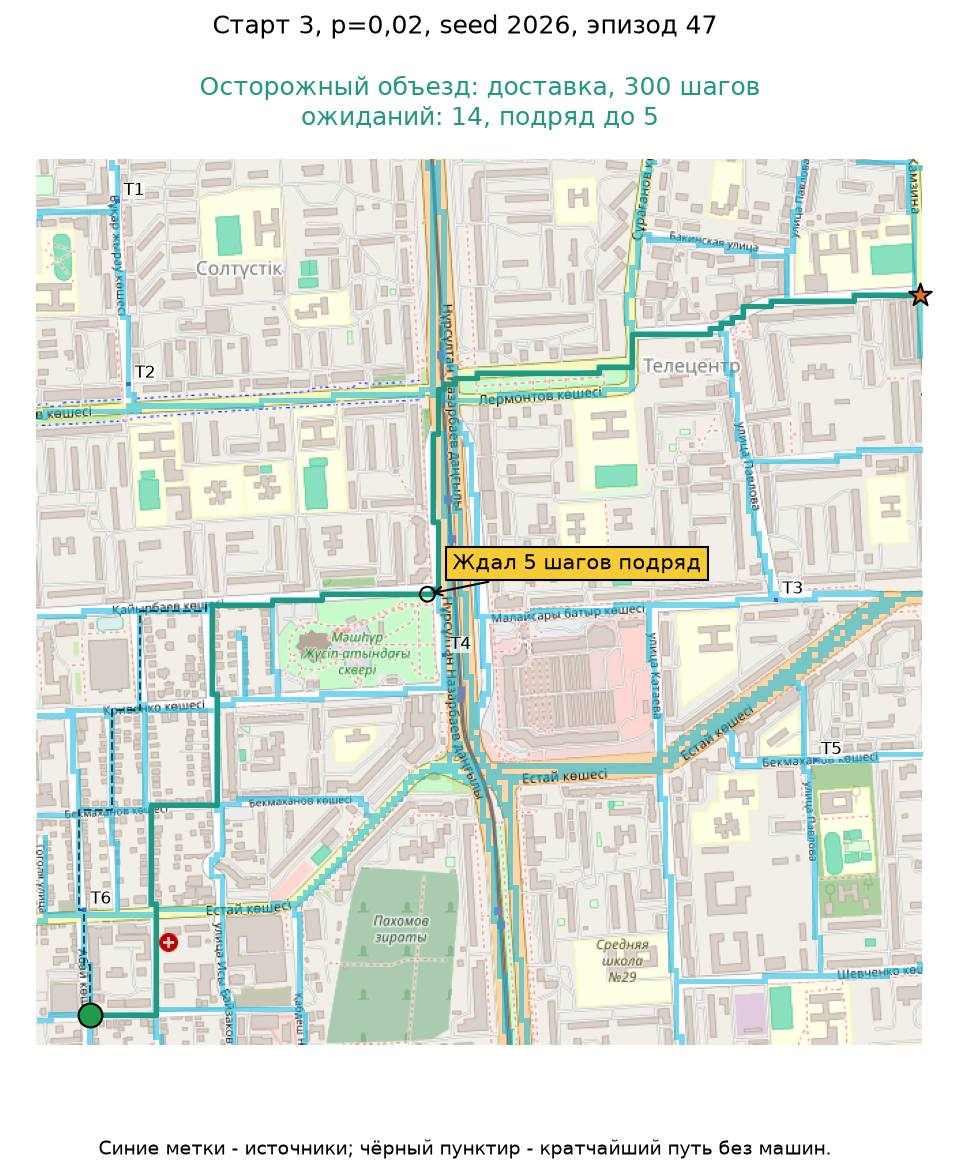
\includegraphics[height=.70\textheight]{start_3_traffic_aware_route.png}
\caption{Осторожный объезд: маршрут со старта 3.}
\end{figure}
\clearpage

\section{Анимации поездок}
В GIF показаны все шаги выбранных удачных и неудачных поездок. Слева находится крупный план, справа - вся карта. Ниже приведены кадры каждого GIF; сами анимированные файлы находятся в каталоге \texttt{results} рядом с ноутбуком.
\begin{figure}[H]
\centering
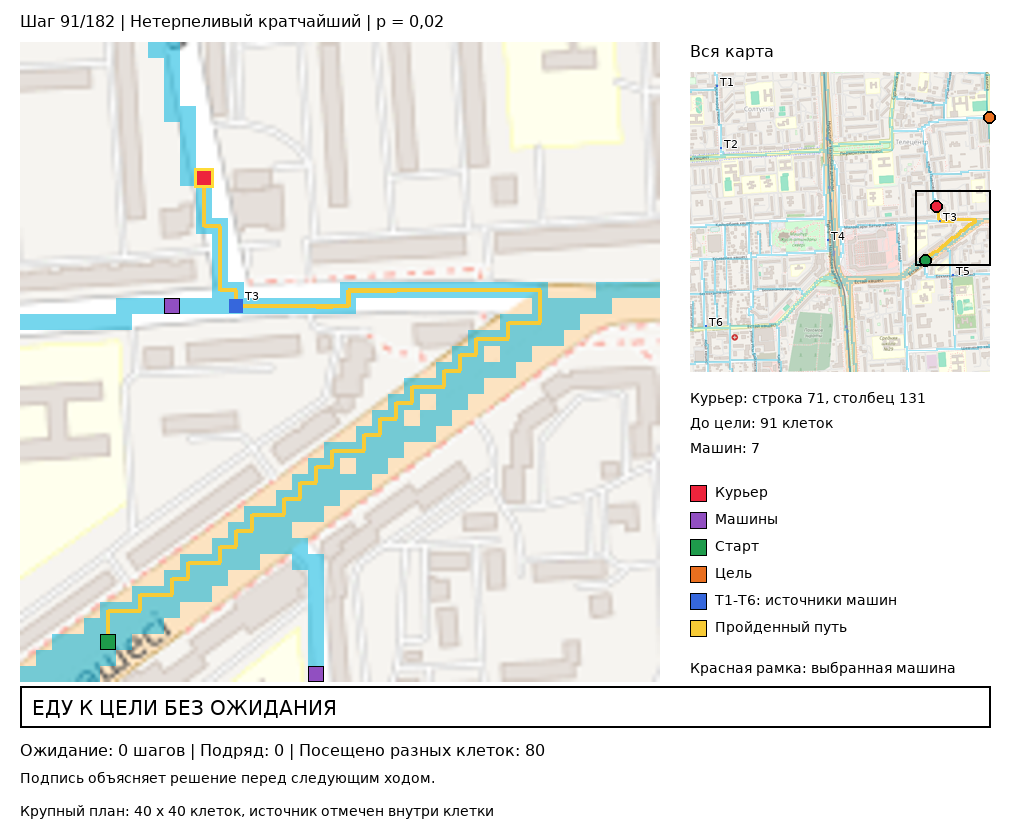
\includegraphics[width=.66\textwidth]{shortest_start2_success_preview.png}
\caption{Нетерпеливый кратчайший: доставка за 182 шага.}
\end{figure}
\begin{figure}[H]
\centering
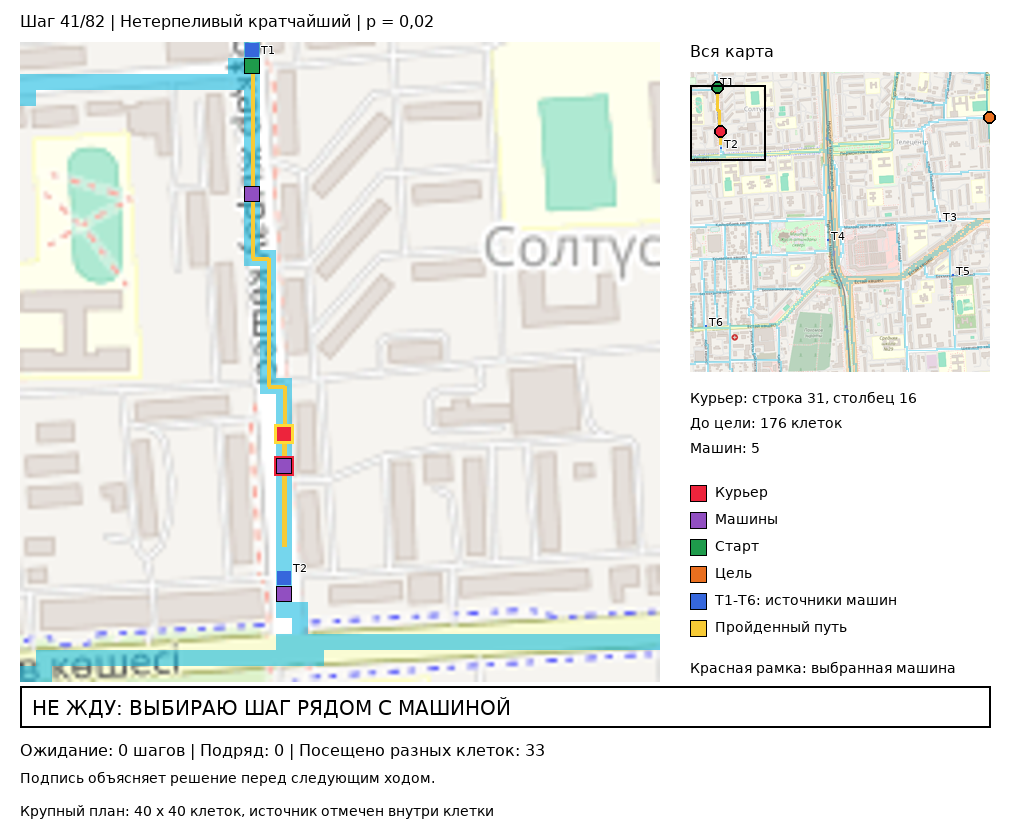
\includegraphics[width=.66\textwidth]{shortest_start1_collision_preview.png}
\caption{Нетерпеливый кратчайший: авария на шаге 82.}
\end{figure}
\begin{figure}[H]
\centering
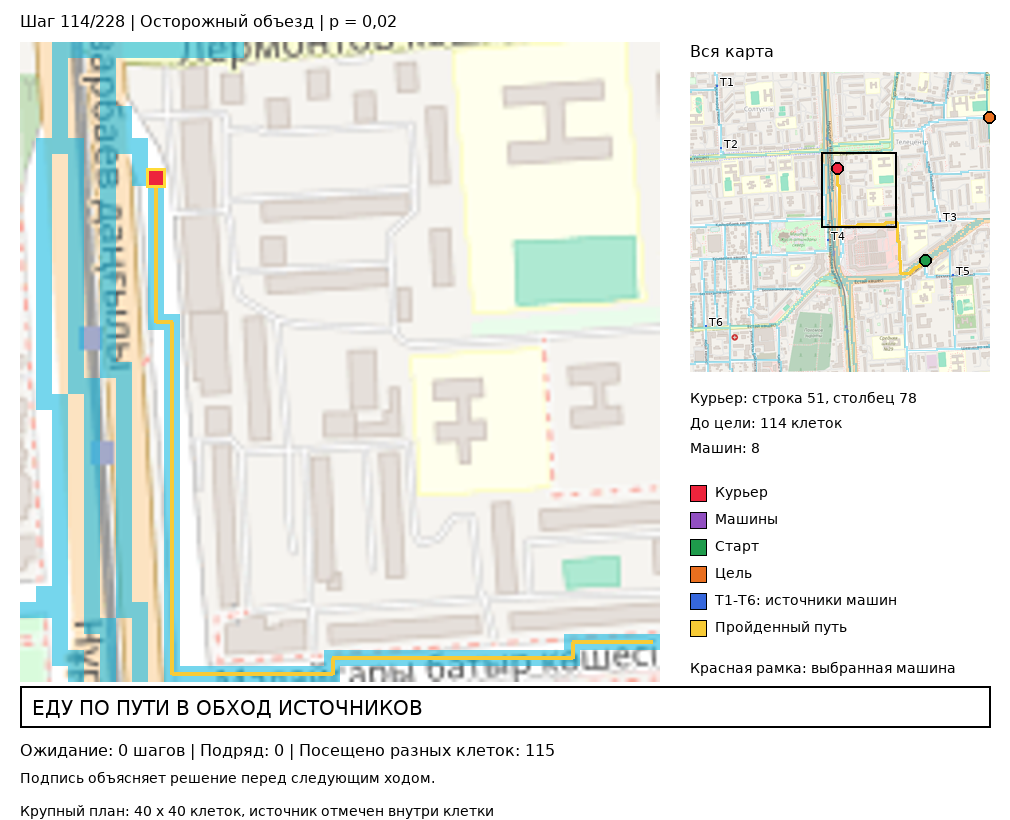
\includegraphics[width=.66\textwidth]{cautious_start2_detour_success_preview.png}
\caption{Осторожный объезд: доставка за 228 шагов.}
\end{figure}
\begin{figure}[H]
\centering
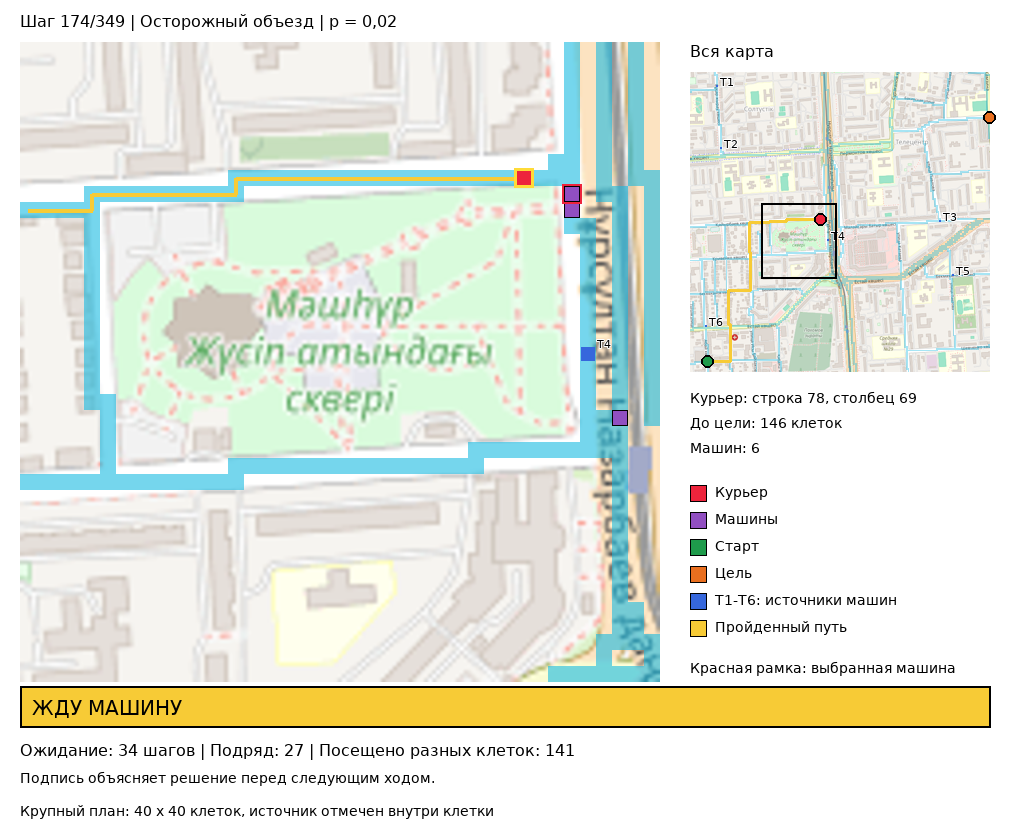
\includegraphics[width=.66\textwidth]{cautious_start3_wait_success_preview.png}
\caption{Осторожный объезд: доставка за 349 шагов, ожидание 61 шаг.}
\end{figure}
\begin{figure}[H]
\centering
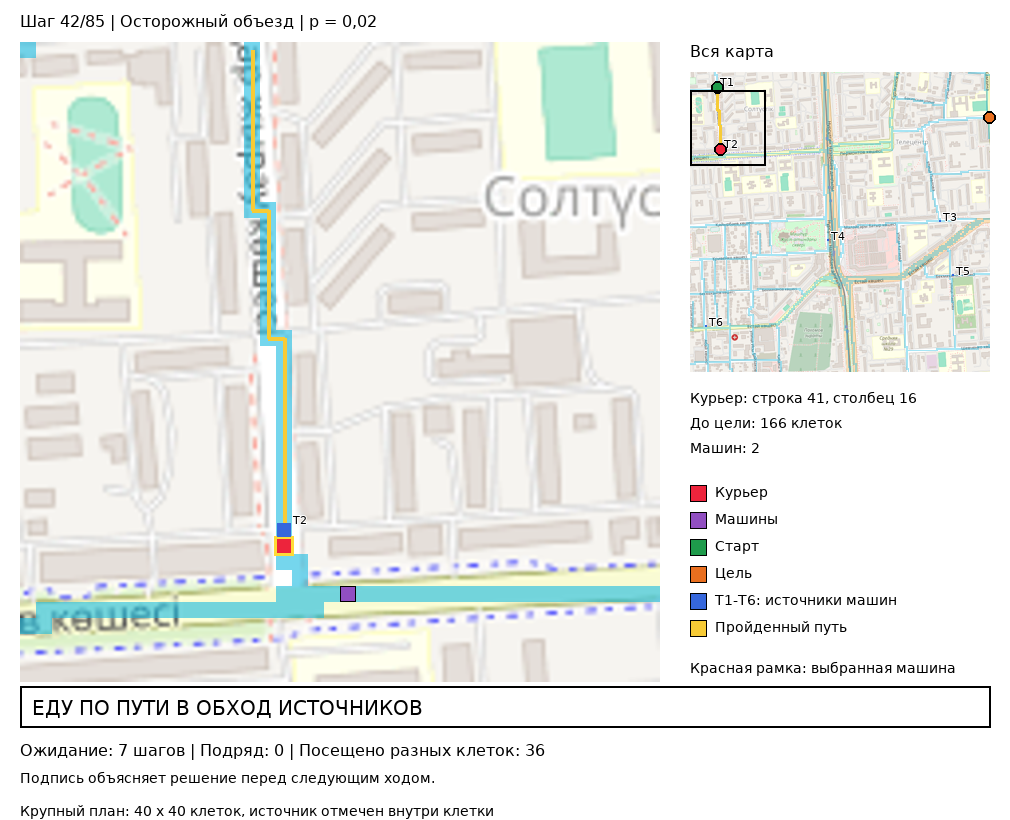
\includegraphics[width=.66\textwidth]{cautious_start1_collision_preview.png}
\caption{Осторожный объезд: авария на шаге 85.}
\end{figure}
\begin{figure}[H]
\centering
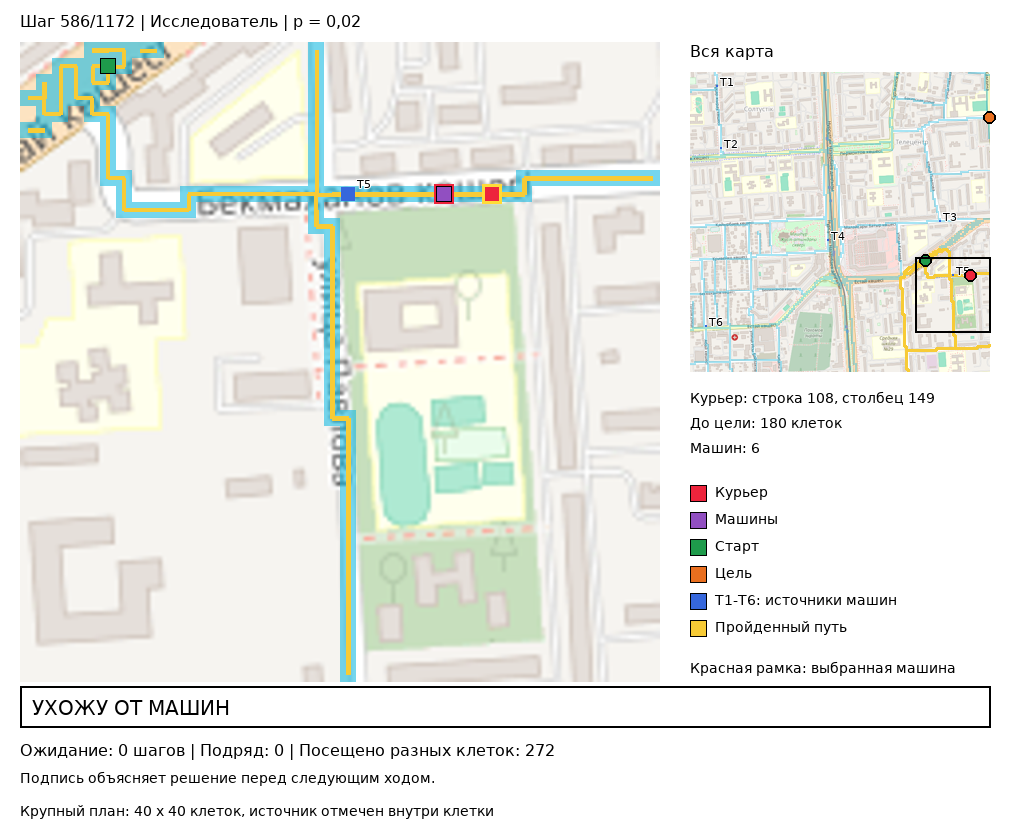
\includegraphics[width=.66\textwidth]{explorer_start2_success_preview.png}
\caption{Исследователь: доставка за 1172 шага.}
\end{figure}
\begin{figure}[H]
\centering
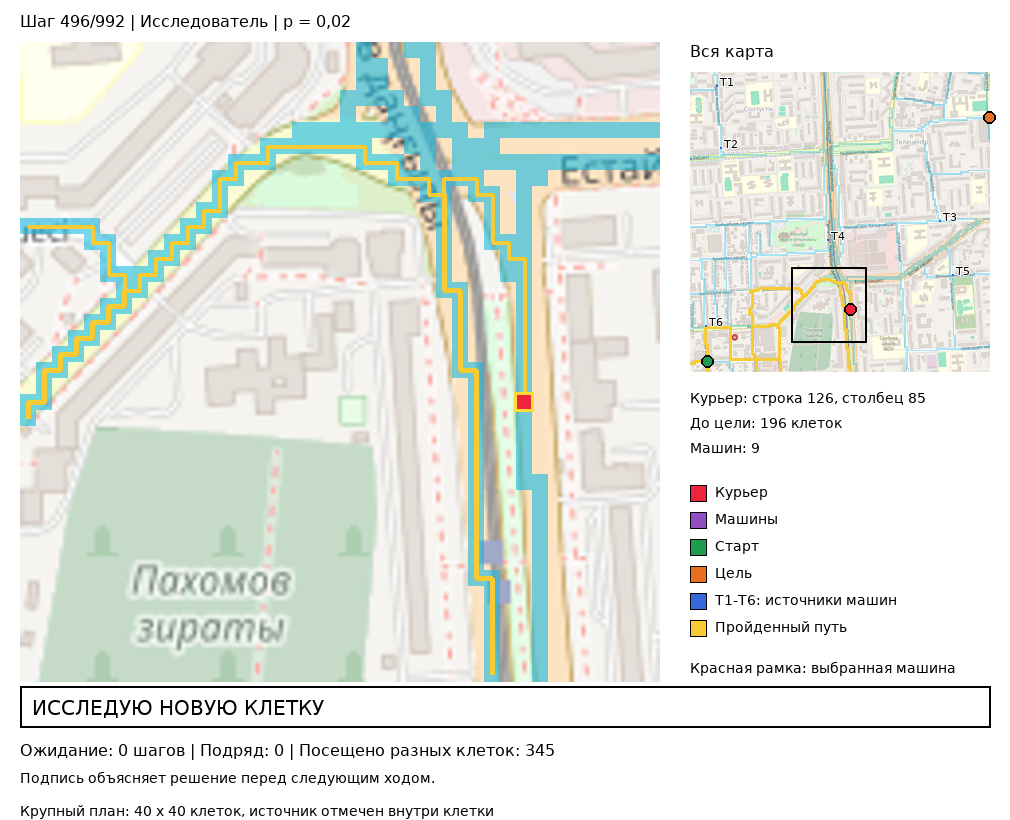
\includegraphics[width=.66\textwidth]{explorer_start3_collision_preview.png}
\caption{Исследователь: авария на шаге 992.}
\end{figure}

\section{Выводы и программный код}
На клеточной карте Павлодара проверены три стратегии курьера при четырёх вероятностях появления машин. Для каждого сочетания вероятности, старта и стратегии проведено 500 поездок с пятью seed; всего --- 18\,000 эпизодов. Без трафика все доставки были успешными. Кратчайшая и осторожная стратегии тогда проходили одинаковое число шагов, а исследователь тратил примерно в 9--15 раз больше из-за поиска новых участков дороги.

При увеличении трафика доля успешных доставок обычно снижалась. При $p=0{,}05$ осторожный объезд доставил 100\% грузов со старта 2 и 99,4\% со старта 3, тогда как кратчайшая стратегия --- 84,2\% и 88,4\%. Со старта 1 обе стратегии получили 78,4\%: преимущество объезда зависит от расположения маршрута и источников машин. У исследователя при той же вероятности доля доставок составила от 32,6\% до 64,6\%.

Среднее число шагов рассчитано только для успешных поездок. Поэтому уменьшение этого показателя у исследователя при росте трафика не означает ускорения: поездки, завершившиеся аварией, в среднее не входят. Анимации показывают поведение в отдельных эпизодах, а выводы о надёжности основаны на всех 500 поездках каждого условия.

Карту строит \texttt{build\_map.py}. Файл \texttt{courier\_project.ipynb} содержит код среды, стратегии, массовый эксперимент, построение всех графиков и GIF с комментариями. Результаты сохранены в \texttt{results/episodes.csv}, \texttt{results/seed\_summary.csv} и \texttt{results/condition\_summary.csv}. Модель приближает улицы клетками и не учитывает реальные правила дорожного движения.
\end{document}
